\documentclass{beamer}
\usepackage{graphics}
\usepackage{epsfig}
\usepackage{multicol}
\usepackage{pifont}
\setbeamertemplate{navigation symbols}{}
\newcommand{\RR}{\ensuremath{\mathbb{R}}}
\newcommand{\NN}{\ensuremath{\mathbb{N}}}
\newcommand{\QQ}{\ensuremath{\mathbb{Q}}}
\newcommand{\CC}{\ensuremath{\mathbb{C}}}
\newcommand{\ZZ}{\ensuremath{\mathbb{Z}}}
\newcommand{\TT}{\ensuremath{\mathbb{T}}}
\newcommand{\HH}{\ensuremath{\mathbb{H}}}
\DeclareMathOperator{\Min}{Min}
\DeclareMathOperator{\Dom}{Dom}
\DeclareMathOperator{\vol}{vol}
\DeclareMathOperator{\Aut}{Aut}
\DeclareMathOperator{\Stab}{Stab}
\DeclareMathOperator{\Sym}{Sym}
\DeclareMathOperator{\Grp}{Grp}
\DeclareMathOperator{\HYP}{HYP}
\DeclareMathOperator{\CUT}{CUT}
\DeclareMathOperator{\GL}{GL}
\DeclareMathOperator{\AGL}{AGL}
\DeclareMathOperator{\Id}{Id}
\DeclareMathOperator{\mint}{min}
\DeclareMathOperator{\vertt}{vert}
\DeclareMathOperator{\conv}{conv}
\DeclareMathOperator{\rank}{rank}

\def\QuotS#1#2{\leavevmode\kern-.0em\raise.2ex\hbox{$#1$}\kern-.1em/\kern-.1em\lower.25ex\hbox{$#2$}}

\begin{document}
\title{Coupling of the Regional Ocean Modeling System (ROMS) and Wind Wave Model}
\author{
\begin{center}
\textcolor{red}{\large \underline{Dutour Sikiri\'c M.}}$^{(1)}$
\textcolor{red}{\large Roland A.}$^{(2)}$
\textcolor{red}{\large Kuzmi\'c M.}$^{(1)}$
\textcolor{red}{\large Janekovi\'c I.}$^{(1)}$
\textcolor{red}{\large Toma\u zi\'c I.}$^{(3)}$\\[2mm]
\end{center}
\begin{flushleft}
(1) \textcolor{blue}{Rudjer Bo\u skovi\'c Institute, Croatia}\\[2mm]
(2) \textcolor{blue}{Technische Universit\"at Darmstadt, Germany}\\[2mm]
(3) \textcolor{blue}{European Space Agency, Darmstadt}
\end{flushleft}
}



\date{\today} 
\frame{\titlepage} 








\frame{
\begin{center}
\begin{tabular*}{7cm}{c}
\\[-0.5cm]
{\Huge \textcolor{blue}{I. }\textcolor{red}{Wave modelling}}
\end{tabular*}
\end{center}
}

\frame{
  \frametitle{Stochastic wave modelling}

\begin{itemize}
\item Oceanic models are using grids (structured or unstructured) of size $1km\leq d\leq 10km$ to simulate the ocean
\item But oceanic waves have a typical wavelength $2m$ $\leq$ $L$ $\leq$ $100m$. So, we cannot resolve waves in the ocean.
\item But if one uses phase averaged models and uses stochastic assumptions
then it is possible to model waves by a spectral wave action density
$N({\bf x},{\bf k})$
\item This density satisfies a Wave Action Equation (\textcolor{red}{WAE}) which represents advection, refraction, frequency shifting and source terms:
\begin{equation*}
\frac{\partial N}{\partial t} + \nabla_x(({\bf c}_g+{\bf u}_A)N) + \nabla_k(\dot{k} N) 
 + \nabla_{\theta}(\dot{\theta} N) = S_{tot}
\end{equation*}
with
\begin{equation*}
S_{tot} = S_{in} + S_{nl3} + S_{nl4} + S_{bot} + S_{ds} + S_{break} + S_{bf}
\end{equation*}
\end{itemize}
}




%\frame{
%  \frametitle{Doppler shift}
%\begin{itemize}
%\item Suppose that we have a uniform current ${\bf u}$ then the dispersion relation is changed to
%\begin{equation*}
%\sigma^2 = g k  \tanh( kh) \mbox{~and~} \omega = \sigma + {\bf k}\cdot {\bf u}
%\end{equation*}
%with $\sigma$ the intrinsic frequency and $\omega$ the absolute frequency.
%\item In the case of a sheared current, the Doppler shift relation changes to
%\begin{equation*}
%\omega = \sigma + {\bf k}\cdot\int_{z=-h}^{z=\xi} {\bf u} \frac{2k\cosh(2k(z+h))}{\sinh(2kD)} dz
%\end{equation*}
%\item The advection velocity ${\bf u}_A$ is usually approximated by the surface current velocity. There is unfortunately no Wave Action Equation in the case of sheared currents.
%\end{itemize}
%}


\frame{
  \frametitle{Wave coupling}

\begin{itemize}
\item Wave models use surface currents for the advection of wave energy and
the free surface enters into the dispersion relation.
\item On the other hand oceanic model can use wave information to:
\begin{itemize}
\item Compute the Stokes drift (current induced by waves, a nonlinear effect).
\item Compute the wave radiation pressure term in the primitive equation.
\item Improve the computation of the surface stress, turbulence.
\item Be used in sediment transport models.
\end{itemize}
\item Thus it makes sense to have oceanic and wave models coupled both ways. We chose to work with the {\tt ROMS} model (a finite difference model) and the {\tt WWM} model (a finite element model by Aron Roland).
\end{itemize}
\begin{center}
\resizebox{4cm}{!}{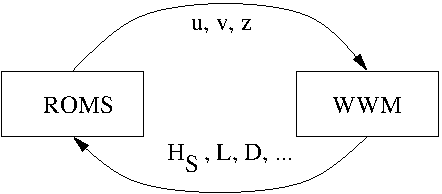
\includegraphics{FIG_wave/Model_Coupling.pdf}}\par
\end{center}
}



\frame{
  \frametitle{The WWM model}
The Wind Wave Model is a third generation wave model authored by Aron Roland and which shares many
common features with WaveWatch III.
\begin{itemize}
\item The Wind Wave Model (WWM) is a unstructured grid spectral wave model.
\item It incorporates most existing source term formulation for wind input and dissipation (Cycle III,
Cycle IV, Ardhuin, Makin, ...)
\item It has been coupled to SELFE, SHYFEM, TIMOR and ROMS.
\item It uses Residual Distribution schemes for the horizontal advection.
\item It integrates the WAE by using the Operator Splitting Method in explicit or implicit mode.
\item It has NETCDF output/input/hotfile.
\item Parallelization is done by ParMETIS.
\end{itemize}
}





\frame{
  \frametitle{Stokes drift}
\begin{itemize}
\item For a complete description, the vertical Stokes drift is needed. It is obtained from the equation
\begin{equation*}
\frac{\partial u_s}{\partial x} + \frac{\partial v_s}{\partial y} + \frac{\partial w_s}{\partial z} = 0
\end{equation*}
and so we can get $w_s$ by vertical integration from the bottom at $z=-h$ to $z=\xi$.
\item For a phase averaged wave model we can compute the horizontal Stokes drift as an integral over the spectrum ($E({\bf k}) = \sigma N({\bf k})$):
\begin{equation*}
(u,v)_{s} = \int_{\bf k} \frac{E({\bf k}) }{2\sinh^2(k(h+\xi))}\sigma {\bf k}\cosh(2k(z+h)) d{\bf k}.
\end{equation*}
Note that the formula is actually an approximation assuming that the current shear is small. See Ardhuin (2008) for higher order formulas.
\end{itemize}
}




\frame{
  \frametitle{Generalized Lagrangian mean}
\begin{itemize}
\item The idea is to decompose the current as ${\bf u}_{tot} = {\bf u} + {\bf u}_{wave} + {\bf u}_{turb}$ with ${\bf u}$ the steady motion, ${\bf u}_{wave}$ the wave motion and ${\bf u}_{turb}$ the microscopic turbulent motion.
\item Under the assumption that ${\bf u}_{turb}$ is uncorrelated to other motion, we have to investigate the relation between ${\bf u}_{wave}$ and ${\bf u}$ (called \textcolor{red}{Quasi-Eulerian}).
\item We can thus introduce a new particular derivative operator
\begin{equation*}
\frac{D}{Dt} = \frac{\partial }{\partial t} + 
(u+u_{S}) \frac{\partial }{\partial x} +
(v+v_{S}) \frac{\partial }{\partial y} +
(w+w_{S}) \frac{\partial }{\partial z}
\end{equation*}
and the equation for tracers $T$ (i.e. salinity, temperature, turbulent kinetic energy, etc.) is then
\begin{equation*}
\frac{D T}{Dt} = S_{source/sink}(T) + S_{diffusion}(T)
\end{equation*}
%with $C(T)$ the source and sink term and $D(T)$ the diffusion term.

\end{itemize}
}





\frame{
  \frametitle{Equations of the Bennis/Ardhuin 2011 formulation I}

\begin{itemize}
\item For the conservation of momentum we have the equation
\begin{equation*}
\frac{D {\bf u}}{D t} = {\bf F}_{pres} + {\bf F}_{turb} + {\bf F}_{cor} + {\bf F}_{wave} + {\bf F}_{bottom} + {\bf F}_{surf}
\end{equation*}
where ${\bf F}_{pres}$ and ${\bf F}_{turb}$ are the pressure and turbulence terms respectively, while ${\bf F}_{cor}=f_{cor} (v + v_s, -u-u_s)$ is the Coriolis term with $f_{cor}$ the Coriolis factor.
\item The wave pressure term is a 
\begin{equation*}
{\bf F}_{wave} = u_s {\bf \nabla} u + v_s {\bf \nabla} v - {\bf \nabla} J
%\left\{\begin{array}{rcl}
%F_{wave, x} &=& \frac{\partial v}{\partial x} v_s + \frac{\partial u}{\partial x} u_s - \frac{\partial J}{\partial x},\\
%F_{wave, y} &=& \frac{\partial v}{\partial y} v_s + \frac{\partial u}{\partial y} u_s - \frac{\partial J}{\partial x}.
%\end{array}\right.
\end{equation*}
with $J$ the 2D wave pressure term given by
\begin{equation*}
J = \int_{\bf k} g\frac{k E({\bf k})}{\sinh(2k (h+\xi))} d{\bf k}
\end{equation*}

\end{itemize}
}





\frame{
  \frametitle{Equations of the Bennis/Ardhuin 2011 formulation II}
\begin{itemize}
\item The equation for the free surface is changed to
\begin{equation*}
\frac{d\xi}{dt} + (u + u_s) \frac{d\xi}{dx} + (v+v_s)\frac{d\xi}{dy} = w + w_s
\end{equation*}
\item Boundary conditions are changed from $u=0$ to $u=-u_s$ and similarly for other kind of boundary conditions.
\item The Stokes drift must also be added to the computation of floats trajectories.
\item (Ardhuin, 2008) actually proposed a more complex system of equations with higher order terms.
\item (Mellor, 2003) proposed some expression for the baroclinic stress but some incoherent results were obtained with it.
\item (Longuet-Higgins, 1953) derived an expression for the barotropic stress induced by waves.


%\item (Ardhuin, 2007) proposed a new set of equations with the basic prototype for the tracer equation:
%\begin{equation*}
%\frac{\partial T}{\partial t} + 
%(u+u_{S}) \frac{\partial T}{\partial x} +
%(v+v_{S}) \frac{\partial T}{\partial y} +
%(w+w_{S}) \frac{\partial T}{\partial z} = S_T
%\end{equation*}
%with $(u,v,w)_S$ being the Stokes drift and $S_T$ the source of the tracer.
%\item The boundary condition for momentum changes from $u=0$ to $u=-u_S$.
\end{itemize}
}







\frame{
  \frametitle{Exchange between Stokes current and current}

\begin{center}
\begin{minipage}{4.6cm}
\centering
\epsfig{file=NCLpictures_drifter/DoNCL_Bennis/Bennis_a_HsB.eps, height=4.2cm}\par
%\resizebox{5.4cm}{!}{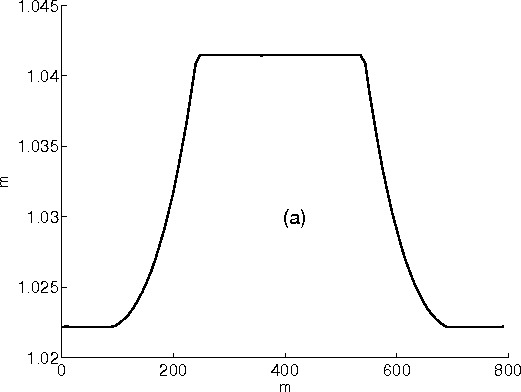
\includegraphics{DrifterPicture/Bennis_second_test/Hwave/Hsignificant18000.jpg}}\par
\end{minipage}
\begin{minipage}{4.6cm}
\centering
\epsfig{file=NCLpictures_drifter/DoNCL_Bennis/Bennis_b_TotalLagB.eps, height=4.2cm}\par
%\resizebox{5.4cm}{!}{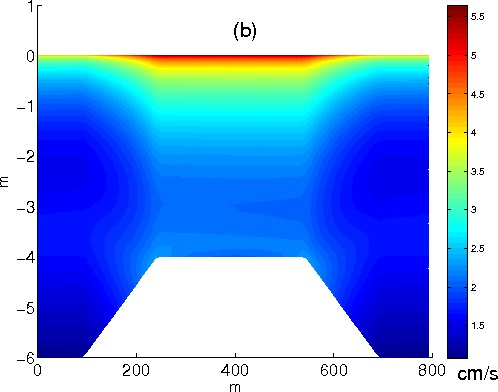
\includegraphics{DrifterPicture/Bennis_second_test/UVlag/Vmagnitude_w18000.jpg}}\par
\end{minipage}
\begin{minipage}{4.6cm}
\begin{itemize}
\item The stokes drift flux is not conservative
\item But the flux $(h+ \xi)(\overline{u} + \overline{u}_s)$ is constant in that test case.
\end{itemize}
\end{minipage}
\begin{minipage}{4.6cm}
\centering
\epsfig{file=NCLpictures_drifter/DoNCL_Bennis/Bennis_c_CurrB.eps, height=4.2cm}\par
%\resizebox{5.4cm}{!}{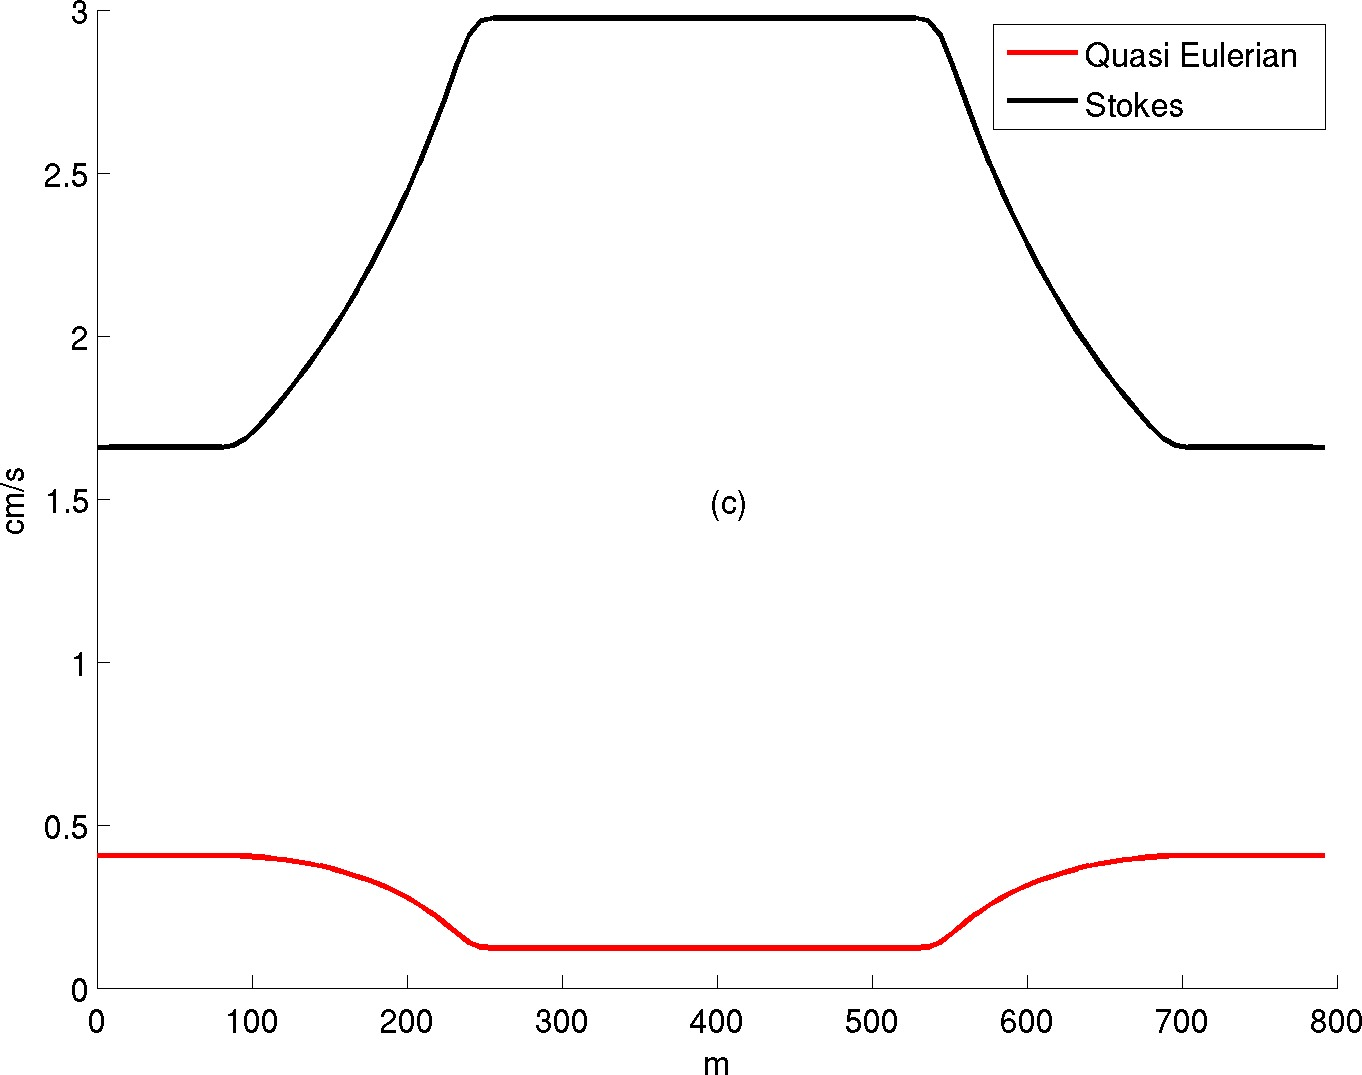
\includegraphics{DrifterPicture/Bennis_second_test/UVbarLag/BaroU_Us18000.jpg}}\par
\end{minipage}
\end{center}
}













\frame{
  \frametitle{Surface stress}
\begin{itemize}
\item Surface stress is a key unknown in many oceanographic simulations.
\item Many formulas depending on the wind ${\bf u}_{10m}$ have been proposed and the Charnock parameter was introduced
\begin{equation*}
\alpha = z_{0,air} \frac{g}{u_{*}^2}
\end{equation*}
with $z_0$ the roughness length and $u_{*}$ the friction velocity. But the variability remains very large.
\item Janssen (1989) proposed to decompose the stress into
\begin{equation*}
\tau = \tau_{viscous}  + \tau_{wave} + \tau_{high.\,freq.}
\end{equation*}
\item The term $\tau_{viscous}$ is negligible. 
\item Janssen (1989) proposed a parameterization of the high frequency stress
\item And $\tau_{wave}$ is obtained as an integral over the wind input formula of the wave model.

\end{itemize}
}




\frame{
\begin{center}
\begin{tabular*}{7cm}{c}
\\[-0.5cm]
{\Huge \textcolor{blue}{II. }\textcolor{red}{Numerical}}\\[4mm]
{\Huge \textcolor{red}{and computer}}\\[4mm]
{\Huge \textcolor{red}{aspects}}
\end{tabular*}
\end{center}
}






%\frame{
%  \frametitle{{\tt MPI} based models}
%\begin{itemize}
%\item Geophysical models are dominated by the {\tt MPI} parallel formalism. In it the program is split into several nodes that communicate by {\tt Recv}/{\tt Send} commands.
%\item As a consequence, when parallelizing models, it is best to have at the beginning an assignment in {\tt MyColor} of the nature of the node, then call
%\begin{center}
%{\tt MPI\_COMM\_SPLIT(MPI\_COMM\_WORLD, MyColor, MyCOMM)}
%\end{center}
%From that point we have a new communicator {\tt MyCOMM} that can be used inside of the existing code by replacing the {\tt MPI\_COMM\_WORLD}
%\item So, apart from exchanging data, merging two {\tt MPI} programs together takes only a few lines.
%\end{itemize}
%}


\frame{
  \frametitle{Model coupling library, {\tt PGMCL} }
\begin{itemize}
\item The exchange between coupled models (via {\tt COMM\_SPLIT}) requires the sending of data between them.
\item A priori the grids are different, the model nature may be different (Structure/Unstructured grids) and so interpolation is needed between the models.
\item There are several existing libraries {\tt MCT}, {\tt OASIS}, {\tt PALM}, etc but when considering them, they appear all relatively complicated.
\item We considered {\tt MCT} and it appeared to be impossible to achieve the goals that we wanted (optimal exchanges, interpolation, performance, etc.).
\item Henceforth, we designed our own library {\tt PGMCL} (Parallel Geophysical Model Coupling Library) for coupling models.
\item After declarations, the commands become as simple as
\begin{center}
{\tt CALL MPI\_INTERP\_SEND(TheArr\_WAVtoOCN, Hwave)}\\
{\tt CALL MPI\_INTERP\_RECV(TheArr\_WAVtoOCN, Hwave)}
\end{center}

\end{itemize}
}




%\frame{
%  \frametitle{Coupling of {\tt WAM} and {\tt COSMO}}
%\begin{itemize}
%\item The {\tt WAM} model, originally the first $3^{rd}$ generation wave model, is a wave model used by many institutions  in the world.
%\item The {\tt COSMO} model is based on the Lokall modell of DWD.
%\item Both are finite difference models that are coupled via {\tt PGMCL}
%\begin{itemize}
%\item The atmospheric model provides the wind and air density to wave model.
%\item The wave model provides the Charnock coefficient to the atmospheric model.
%\end{itemize}
%\item Results on the Mediterranean indicate a slight decrease of wind magnitude.
%\end{itemize}
%Work done in collaboration with P. Janssen/J. Bidlot (ECMWF), L. Cavaleri (ISMAR), L. Torrisi (CNMCA, Italian Nat. Met. Center) and A. Roland (TU Darmstadt)
%}






%\frame{
%  \frametitle{WaveWatch III coarse/fine grids}
%\begin{itemize}
%\item The WaveWatch III model is another wave model used by several oceanographic institutions. It can work with nested grids, which are finite difference or finite element.
%\item My contribution was the implementation of coarse $\rightarrow$ fine (interpolation) and fine $\rightarrow$ coarse (averaging, scrip library) in the case (FD/FE).
%\end{itemize}
%\begin{center}
%\begin{minipage}{3.9cm}
%\centering
%\resizebox{3.9cm}{!}{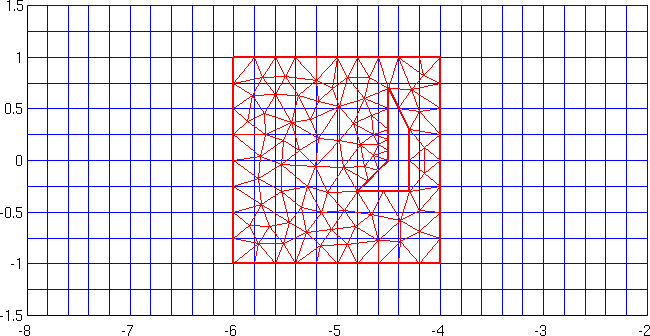
\includegraphics{WavePic/MultiFD_FE_atp5/MultGrid.png}}\par
%\end{minipage}
%\begin{minipage}{3.3cm}
%\centering
%\resizebox{3.3cm}{!}{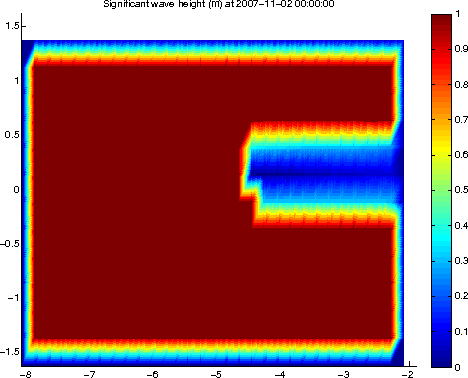
\includegraphics{WavePic/MultiFD_FE_atp5/FD_Hwave_ww0009_20071102_000000.png}}\par
%\end{minipage}
%\begin{minipage}{3.3cm}
%\centering
%\resizebox{3.3cm}{!}{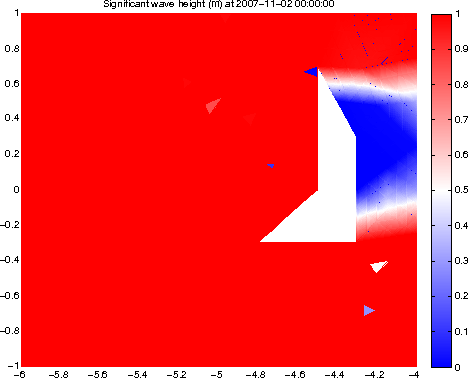
\includegraphics{WavePic/MultiFD_FE_atp5/FE_Hwave_ww0009_20071102_000000.png}}\par
%\end{minipage}
%\end{center}
%Work done with F. Ardhuin (IFREMER), E. Rogers (NRL) and A. Roland (TU Darmstadt)
%}




\frame{
  \frametitle{Numerics of the coupling I}
\begin{itemize}
\item The mathematical expressions occurring in wave coupling theories are dangerous expressions like:
\begin{equation*}
\frac{\cosh(2k (z+h))}{\sinh(2k (h+\xi))}
\end{equation*}
\item This kind of function is very singular. Their large values are concentrated on the surface. On the other hand it satisfies a specific integral property:
\begin{equation*}
\frac{1}{h+\xi} \int_{-h}^{\xi} \frac{\cosh(2k (z+h))}{\sinh(2k (h+\xi))} dz=\frac{1}{2k(h+\xi)}
\end{equation*}
which has to be reproduced in the model.
\item The solution that we choose is for every vertical cell of the model, to compute explicitly the integral and put the average value at the relevant point.
\item We also use a $k_{eff} = \frac{1}{D} \min(300, k(h+\xi))$.
\end{itemize}
}


\frame{
  \frametitle{Numerics of the coupling II}
\begin{itemize}
\item For the Stokes drift the model value for a vertical cell between depth $z$ and $z'$ is
\begin{equation*}
\begin{array}{rcl}
(u_s^{model}, v_s^{model})
&=& \frac{1}{z' - z}\int_k \int_z^{z'} (u_s, v_s) dz dk = (*)\\
\end{array}
\end{equation*}
\item After computation this gives:
\begin{equation*}
\begin{array}{rcl}
(*) &=& \int_k \sigma {\bf k} E(k)dk  \frac{1}{\sinh^2(k(h+\xi))} \frac{\sinh(2k(z'+h)) - \sinh(2k(z+h))}{2k(z'-z)}\\
\end{array}
\end{equation*}
\item After simplification this gives:
\begin{equation*}
\begin{array}{rcl}
(*) &=& \int_k \sigma {\bf k} E(k) dk \frac{\cosh(kz+kz' + 2kh)}{\sinh^2(k(h+\xi))}  \textcolor{red}{\frac{\sinh(k(z' - z))}{k(z'-z)}}
\end{array}
\end{equation*}
which is numerically stable.
\item If one does not add the final part then the baroclinic Stokes drift does not match the analytical value.
\end{itemize}
}




\frame{
  \frametitle{Computation of the Stokes drift}

\begin{center}
\begin{minipage}{5.0cm}
\centering
\resizebox{4.4cm}{!}{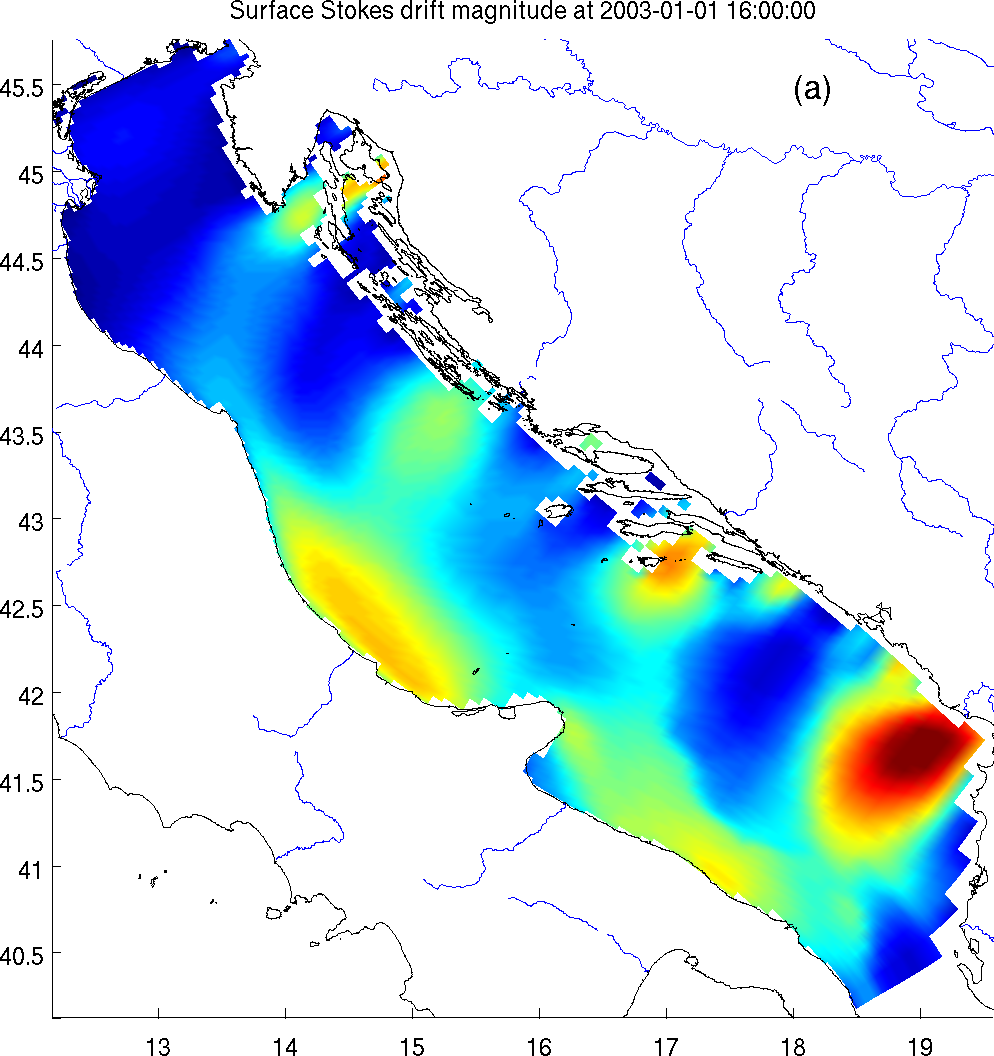
\includegraphics{DrifterPicture/TRC_Stokes_mod.png}}\par
\end{minipage}
\begin{minipage}{5.3cm}
\centering
\resizebox{5.0cm}{!}{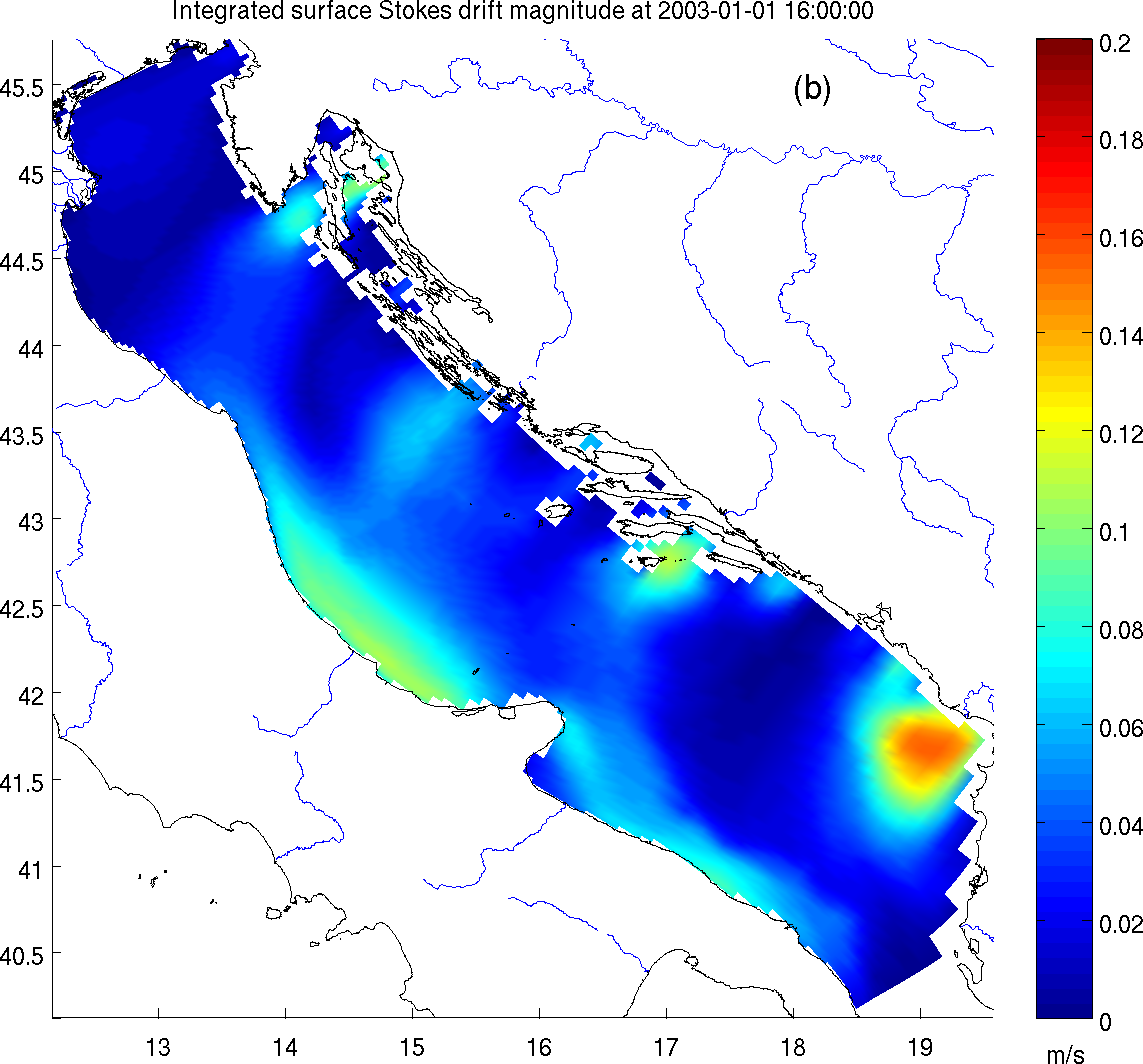
\includegraphics{DrifterPicture/INT_Stokes.png}}\par
\end{minipage}
\end{center}
\begin{itemize}
\item For $N_{freq}$ frequencies, $N_{dir}$ directions, $N_{vert}$ vertical levels and $N_{node}$ grid level points the computation of the Stokes drift is takes  $N_{freq}\times N_{dir}\times N_{vert}\times N_{node}$ operations.
\item We can reduce it to $N_{node}\times N_{freq} \times (N_{dir} + N_{vert})$.
\item Truncation formulation is comparable in complexity.
\end{itemize}
}






\frame{
  \frametitle{Grid subdivizion schemes}
\begin{itemize}
\item Our standard interpolation strategy is to subdivide the squares in two triangles. Then near the coast, we add some more triangles.
\begin{center}
\begin{minipage}{3.2cm}
\centering
\resizebox{2.5cm}{!}{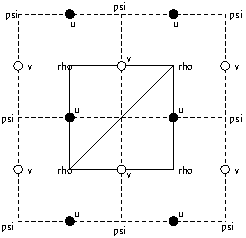
\includegraphics{FIG_wave/Subdiv_straightforward_red.pdf}}\par
\end{minipage}
\begin{minipage}{3.2cm}
\centering
\rotatebox{90}{\resizebox{2.5cm}{!}{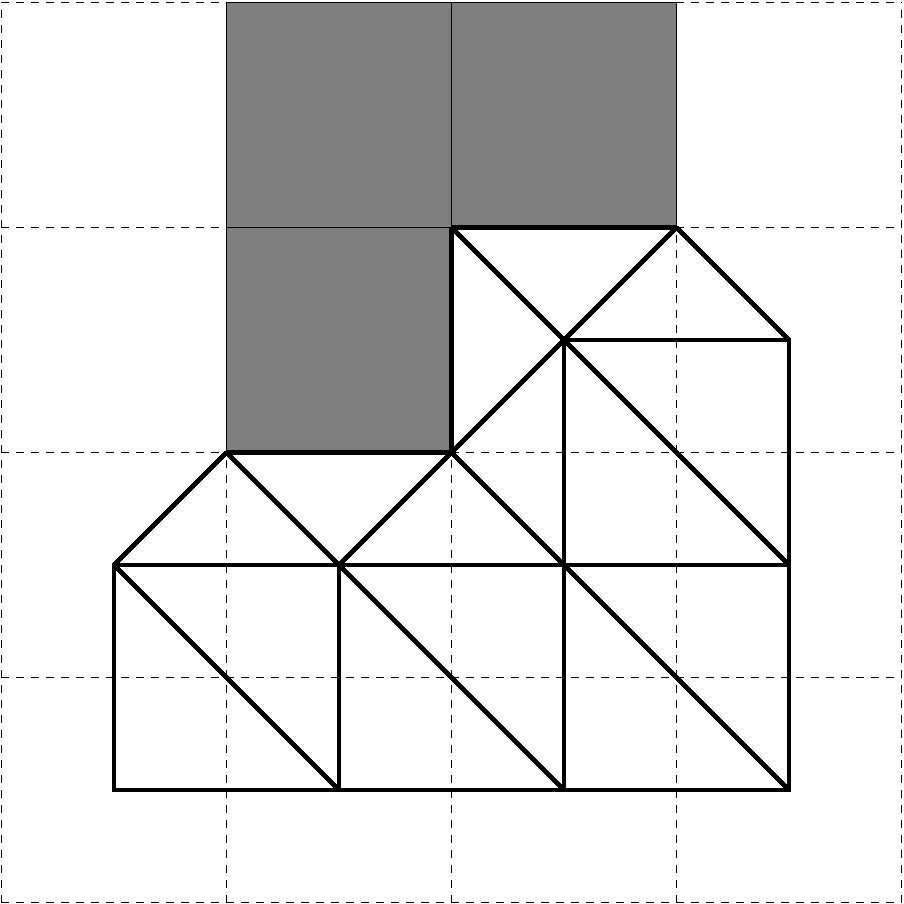
\includegraphics{FIG_wave/Subdiv_coast.pdf}}}\par
\end{minipage}
\end{center}
\item Those additional triangles allow us to respect the straits and isthmus of the original grid.
\begin{center}
\begin{minipage}{3.2cm}
\centering
\rotatebox{90}{\resizebox{2.5cm}{!}{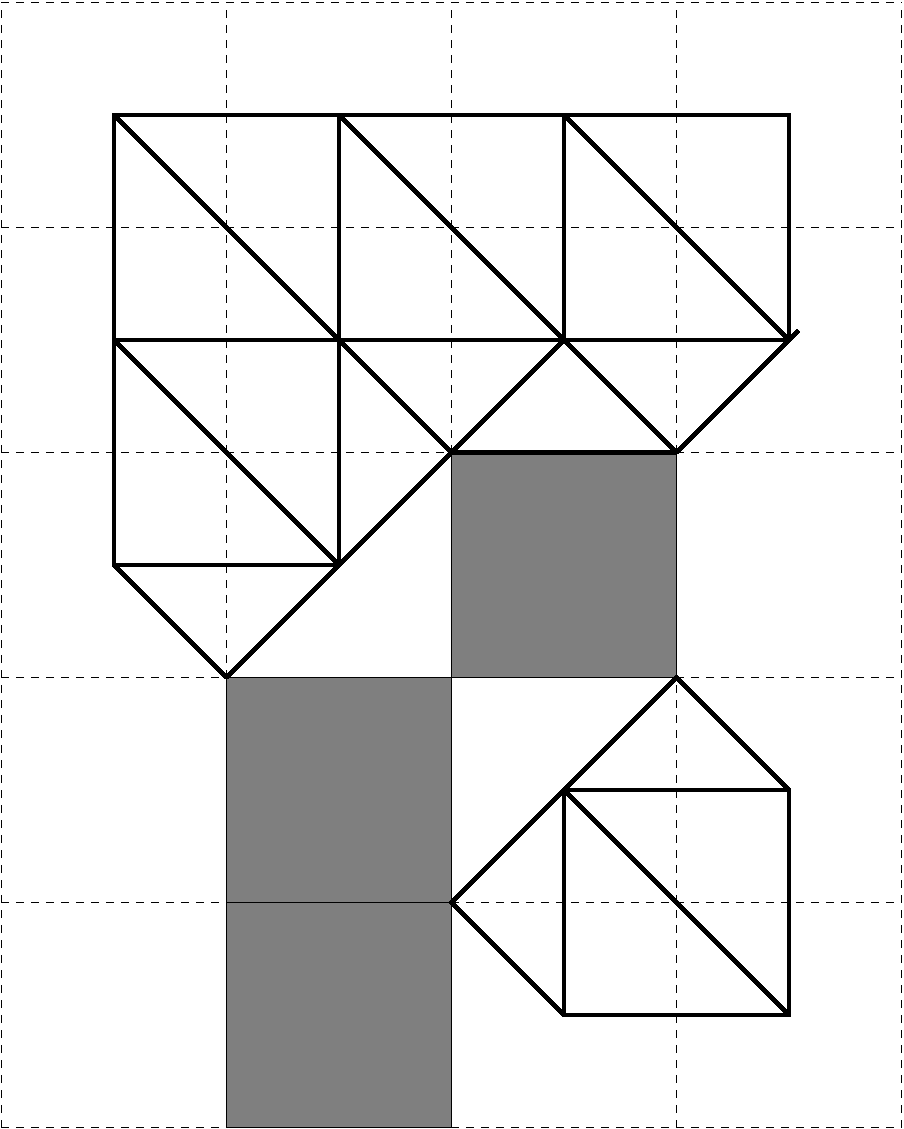
\includegraphics{FIG_wave/Subdiv_isthmus.pdf}}}\par
\end{minipage}
\begin{minipage}{3.2cm}
\centering
\rotatebox{90}{\resizebox{2.5cm}{!}{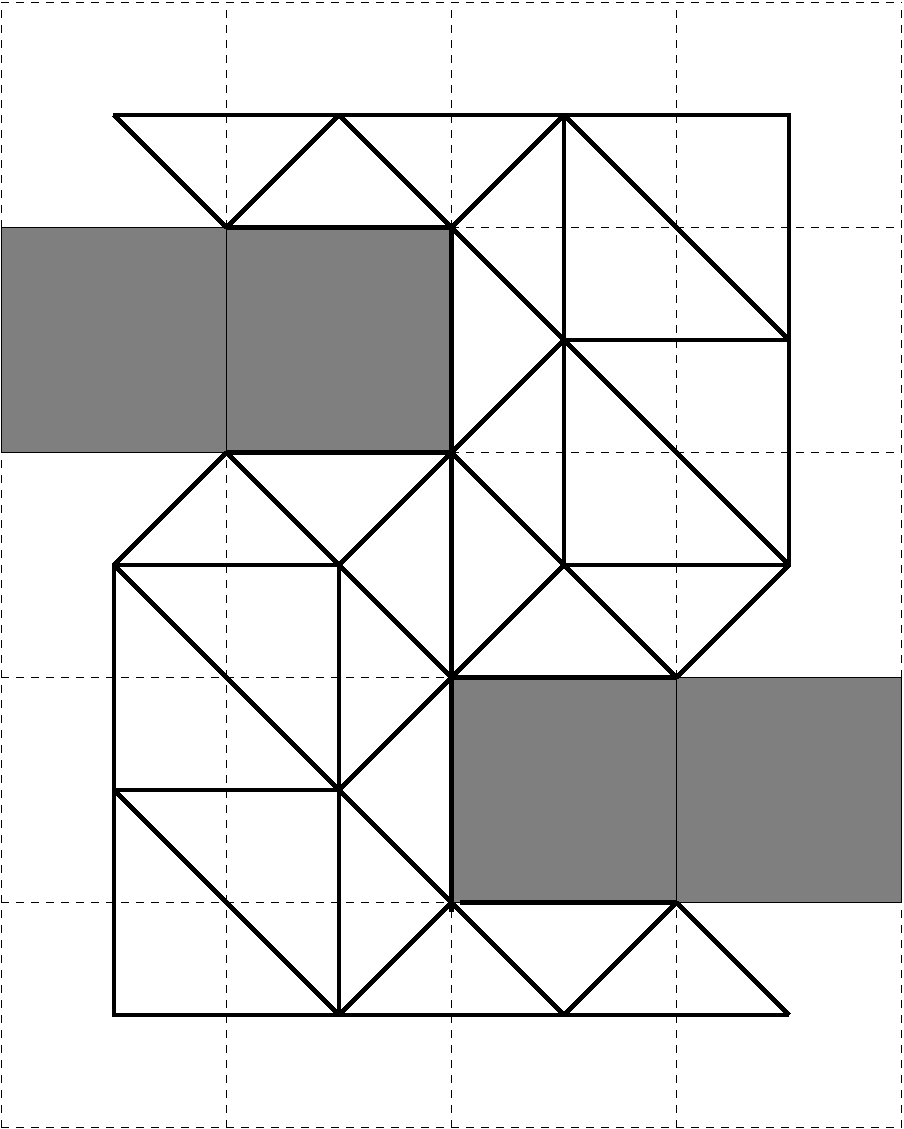
\includegraphics{FIG_wave/Subdiv_strait.pdf}}}\par
\end{minipage}
\end{center}
\item But the system also allows some finite element grid to be used.
\end{itemize}
}

















\frame{
\begin{center}
\begin{tabular*}{6cm}{c}
\\[-0.5cm]
{\Huge \textcolor{blue}{III. }\textcolor{red}{Application to}}\\[4mm]
{\Huge \textcolor{red}{the Adriatic Sea}}
\end{tabular*}
\end{center}
}


\frame{
  \frametitle{Bathymetry and rivers of the Adriatic Sea}

\begin{itemize}
\item The bathymetry varies a lot from 1200m to 50m.
\item The island structure on the Croatian side is quite complex.
\item River inflow is more important than in other parts of the Mediterranean.
\end{itemize}

\begin{center}
\begin{minipage}[b]{5.3cm}
%l b r t
\resizebox{5.2cm}{!}{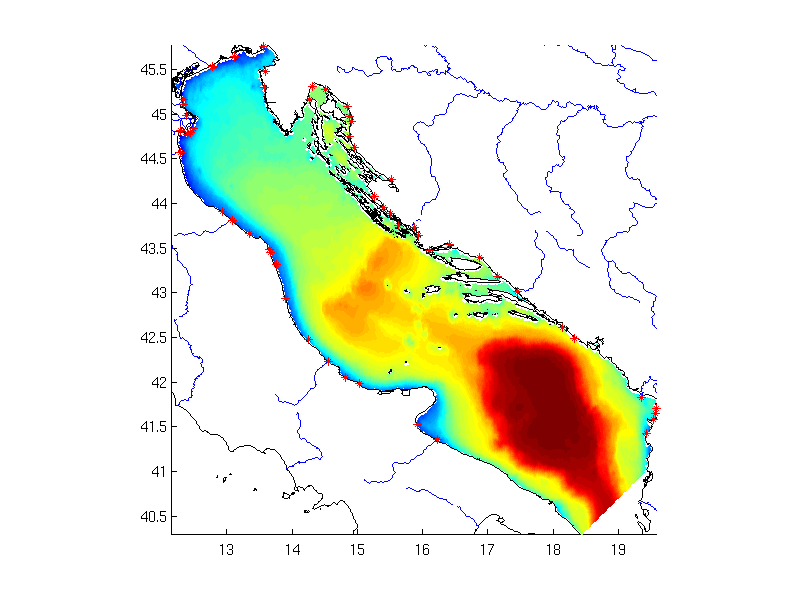
\includegraphics[trim=35mm 11mm 35mm 11mm, clip]{PictureElect/BathymetryRiver.png}}\par
%\resizebox{5.5cm}{!}{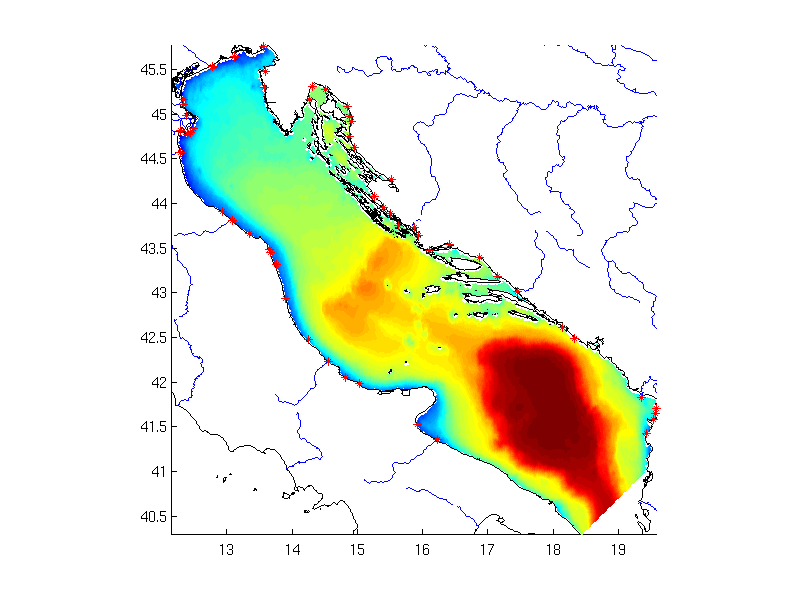
\includegraphics[bb=101 32 477 403, clip]{PictureElect/BathymetryRiver.pdf_V1}}\par
\end{minipage}
\begin{minipage}[b]{5.3cm}
\begin{itemize}
\item Significant inflow/outflow occurs at the Ottranto strait and generates the highest tides of the Mediterranean.
\item Two winds bora and Sirocco dominate the general circulation.
\end{itemize}
\end{minipage}
\end{center}

}




%\frame{
%  \frametitle{General circulation in the Adriatic Sea}
%
%\begin{itemize}
%\item The Mediterranean Sea exerts a significant influence at the Ottranto strait on the general circulation in the Adriatic.
%\item The tides are the highest in the Mediteranean sea.
%\end{itemize}
%}

%\frame{
%  \frametitle{A grid and the bathymetry}
%NEED TO CLEAN the HIGHER PART AND PUT gradation
%\vspace{-0.4cm}
%\begin{center}
%\resizebox{10.0cm}{!}{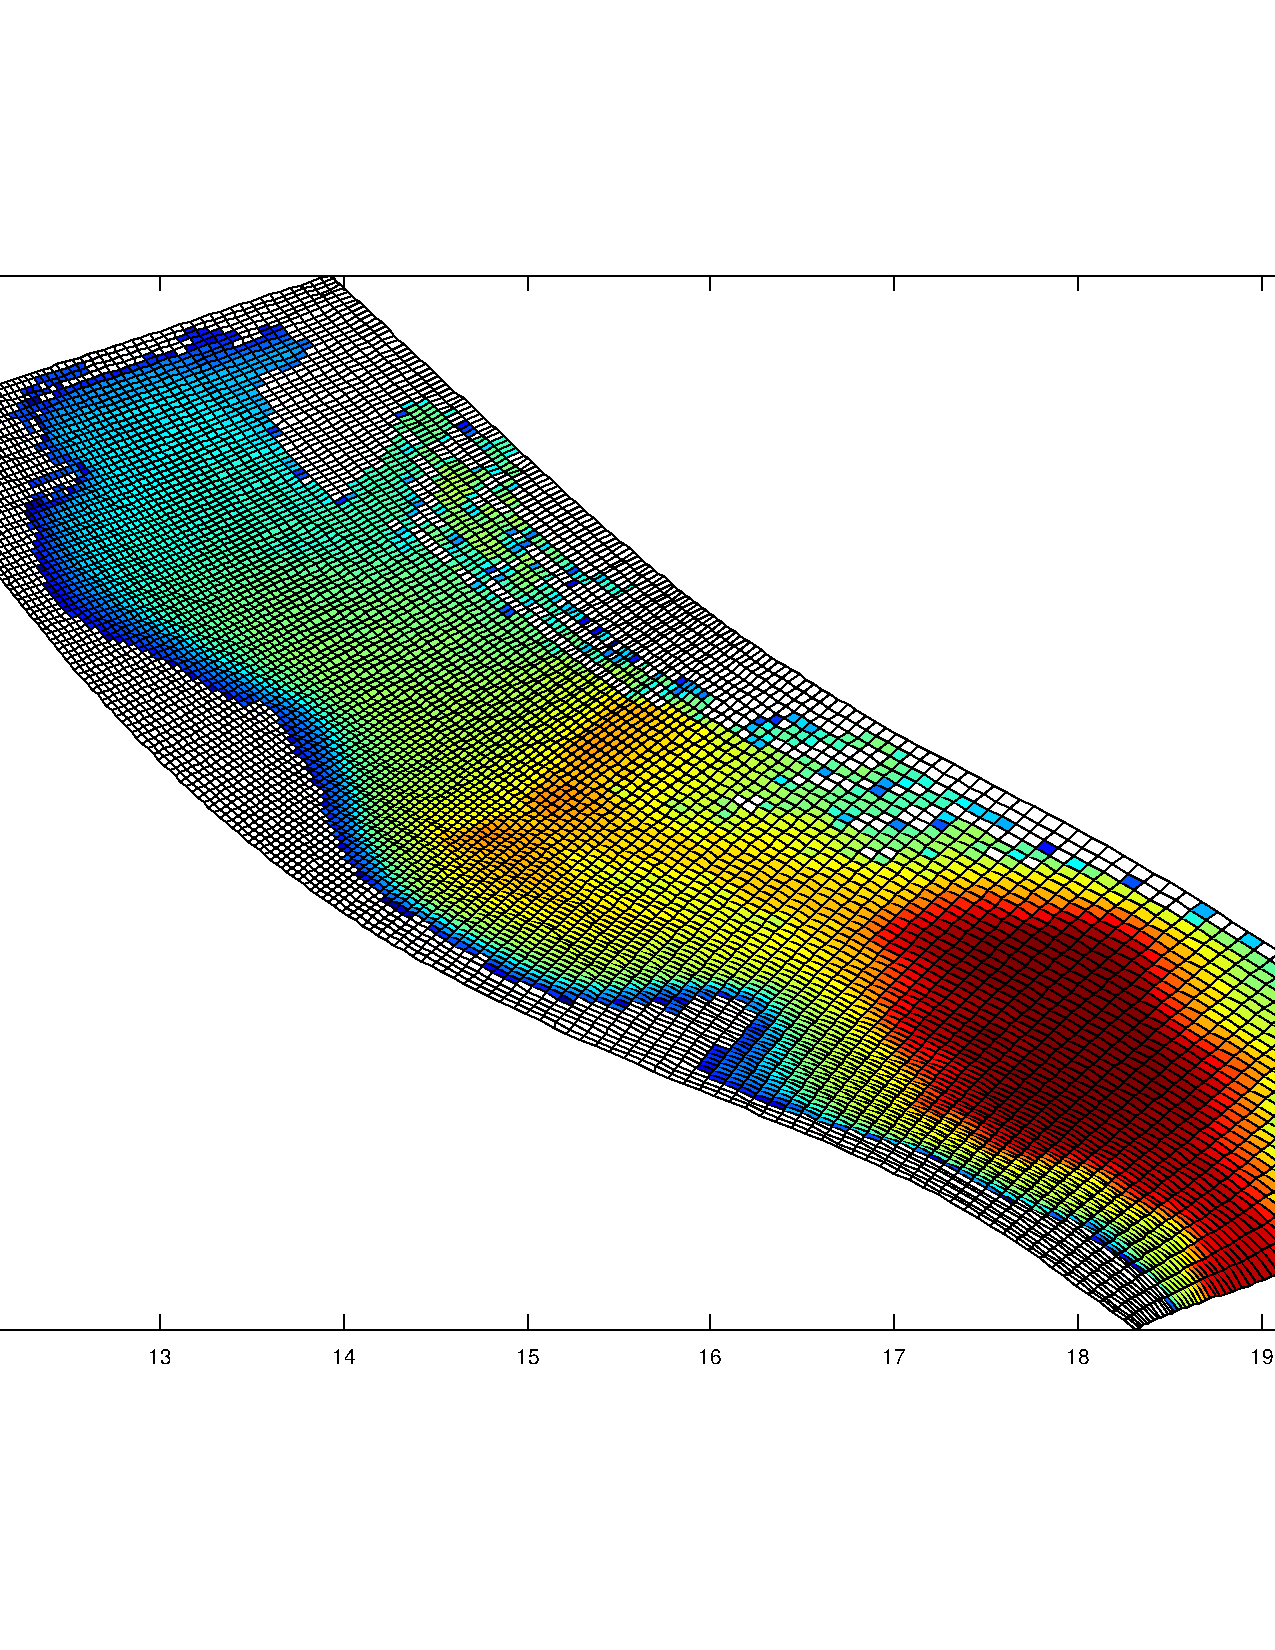
\includegraphics[bb=0 165 612 649, clip]{OceanPic/LogGridRich.pdf}}\par
%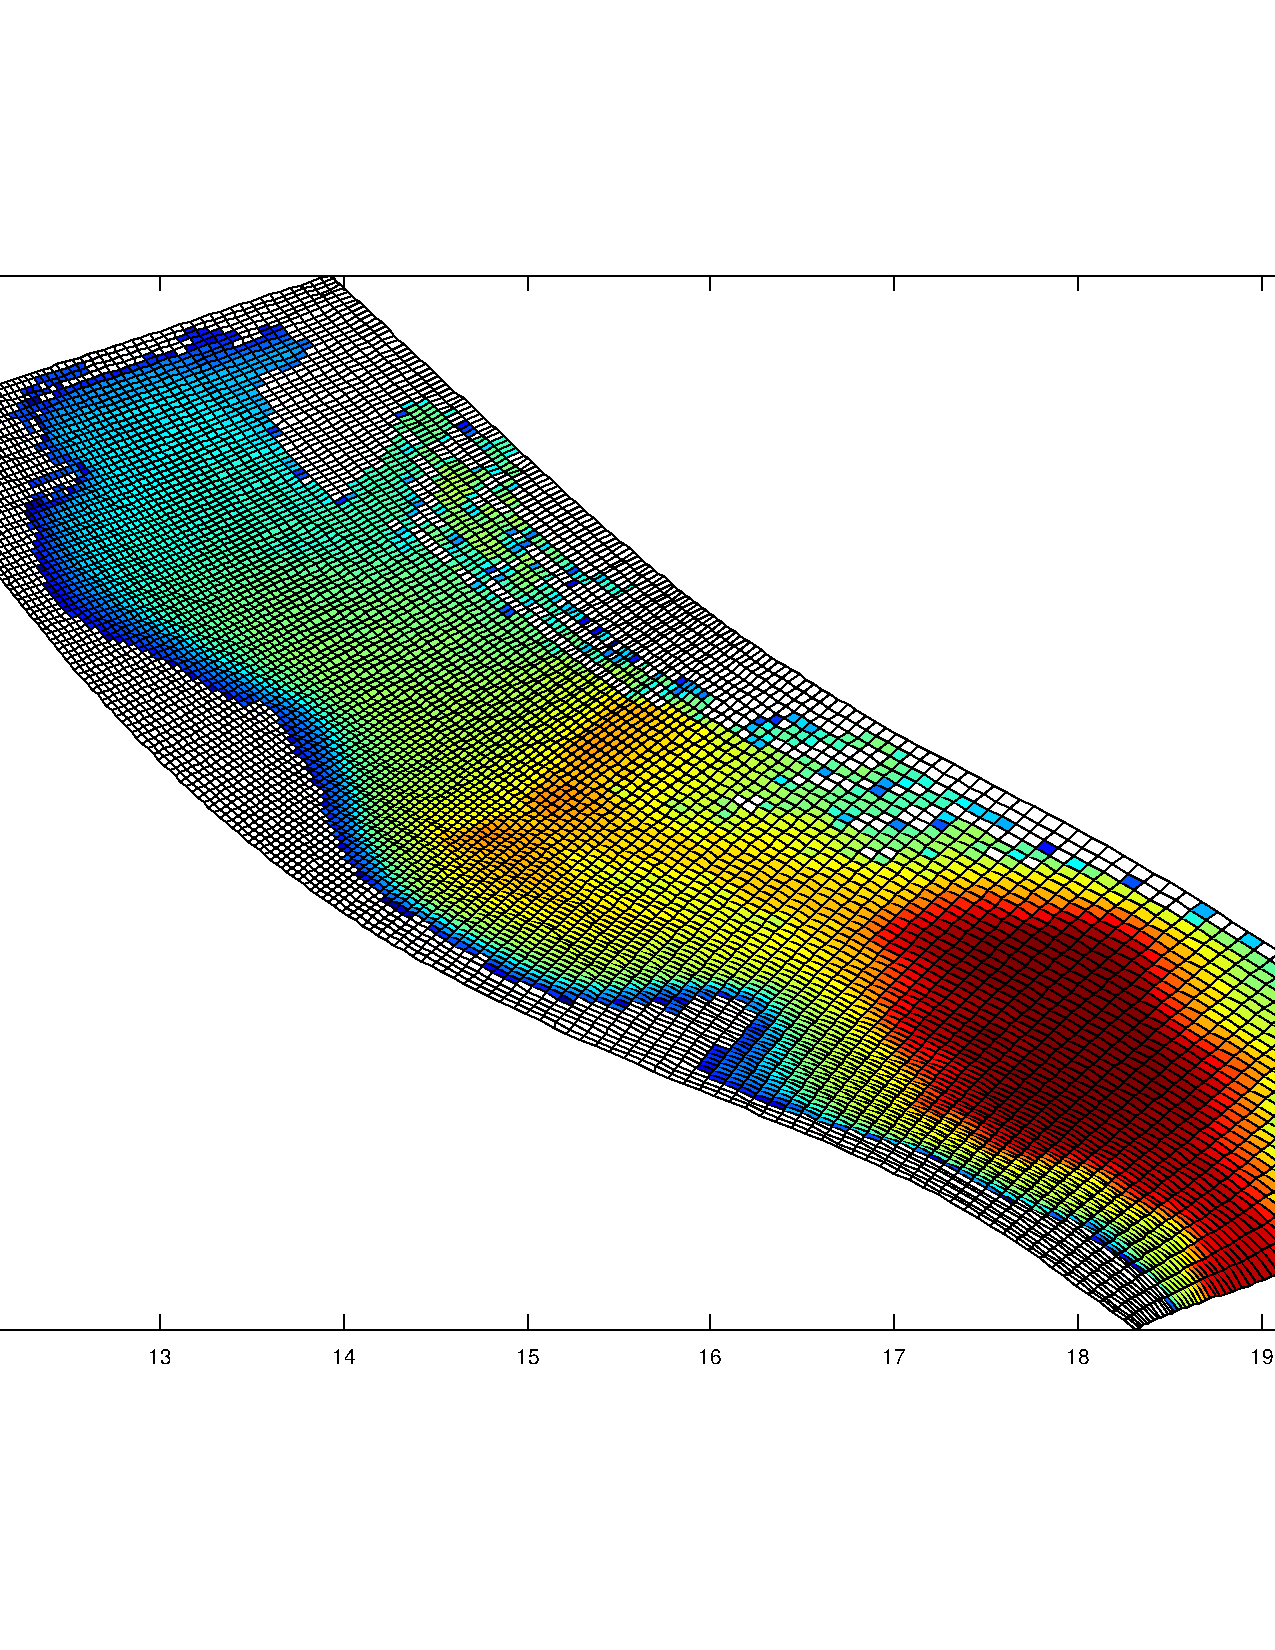
\epsfig{file=OceanPic/LogGridRich.pdf, height=13cm}
%\end{center}
%}



\frame{
  \frametitle{Chosen forcing information}

\begin{itemize}
\item The chosen modelization of the Adriatic Sea uses the atmospheric forcing fields from {\tt DHMZ} using the {\tt ALADIN} model (sea surface pressure, temperature, humidity, rain, cloud factor, short wave radiation).
\item For river forcing, we used:
\begin{itemize}
\item Hourly measurements for Po river and Neretva river.
\item Daily flux measurements for 9 other rivers and temperature for 5 more.
\item For other Italian rivers, we used climatological information from Raicich, 1994. For other Croatian rivers we rescale according to Neretva inflow.
\item For temperature we took nearest river.
\end{itemize}
\item We used an initial state obtained from {\tt AREG} which is an operational model using a modification of {\tt POM}.
\item At the open boundary of the Ottranto strait, we used daily average from the {\tt AREG} model and we add tidal signal to it.
\end{itemize}
}





%\frame{
%  \frametitle{Available measurements}
%
%\begin{itemize}
%\item Satellite \textcolor{blue}{AVHRR} measurements sea surface temperature are available every few hours but are affected by clouds.
%\item Daily \textcolor{blue}{Medspiration} synthetic data sets at 2km resolution of foundation temperature are created from various mea\-su\-re\-ments and model output. {\tt RMSE} is about $0.4 deg$.
%\item {\em In situ} \textcolor{blue}{CTD} measurements available from cruises (Nov 2007, Mar, Jun, Jul 2008) with a priori insignificant error.
%\item Sea level gauges are available.
%\item ADCP (Acoustic Doppler Current Profiler) measures of currents.
%\item Output of meteorological models are available to get forcing data.
%\end{itemize}
%\begin{center}
%\resizebox{4cm}{!}{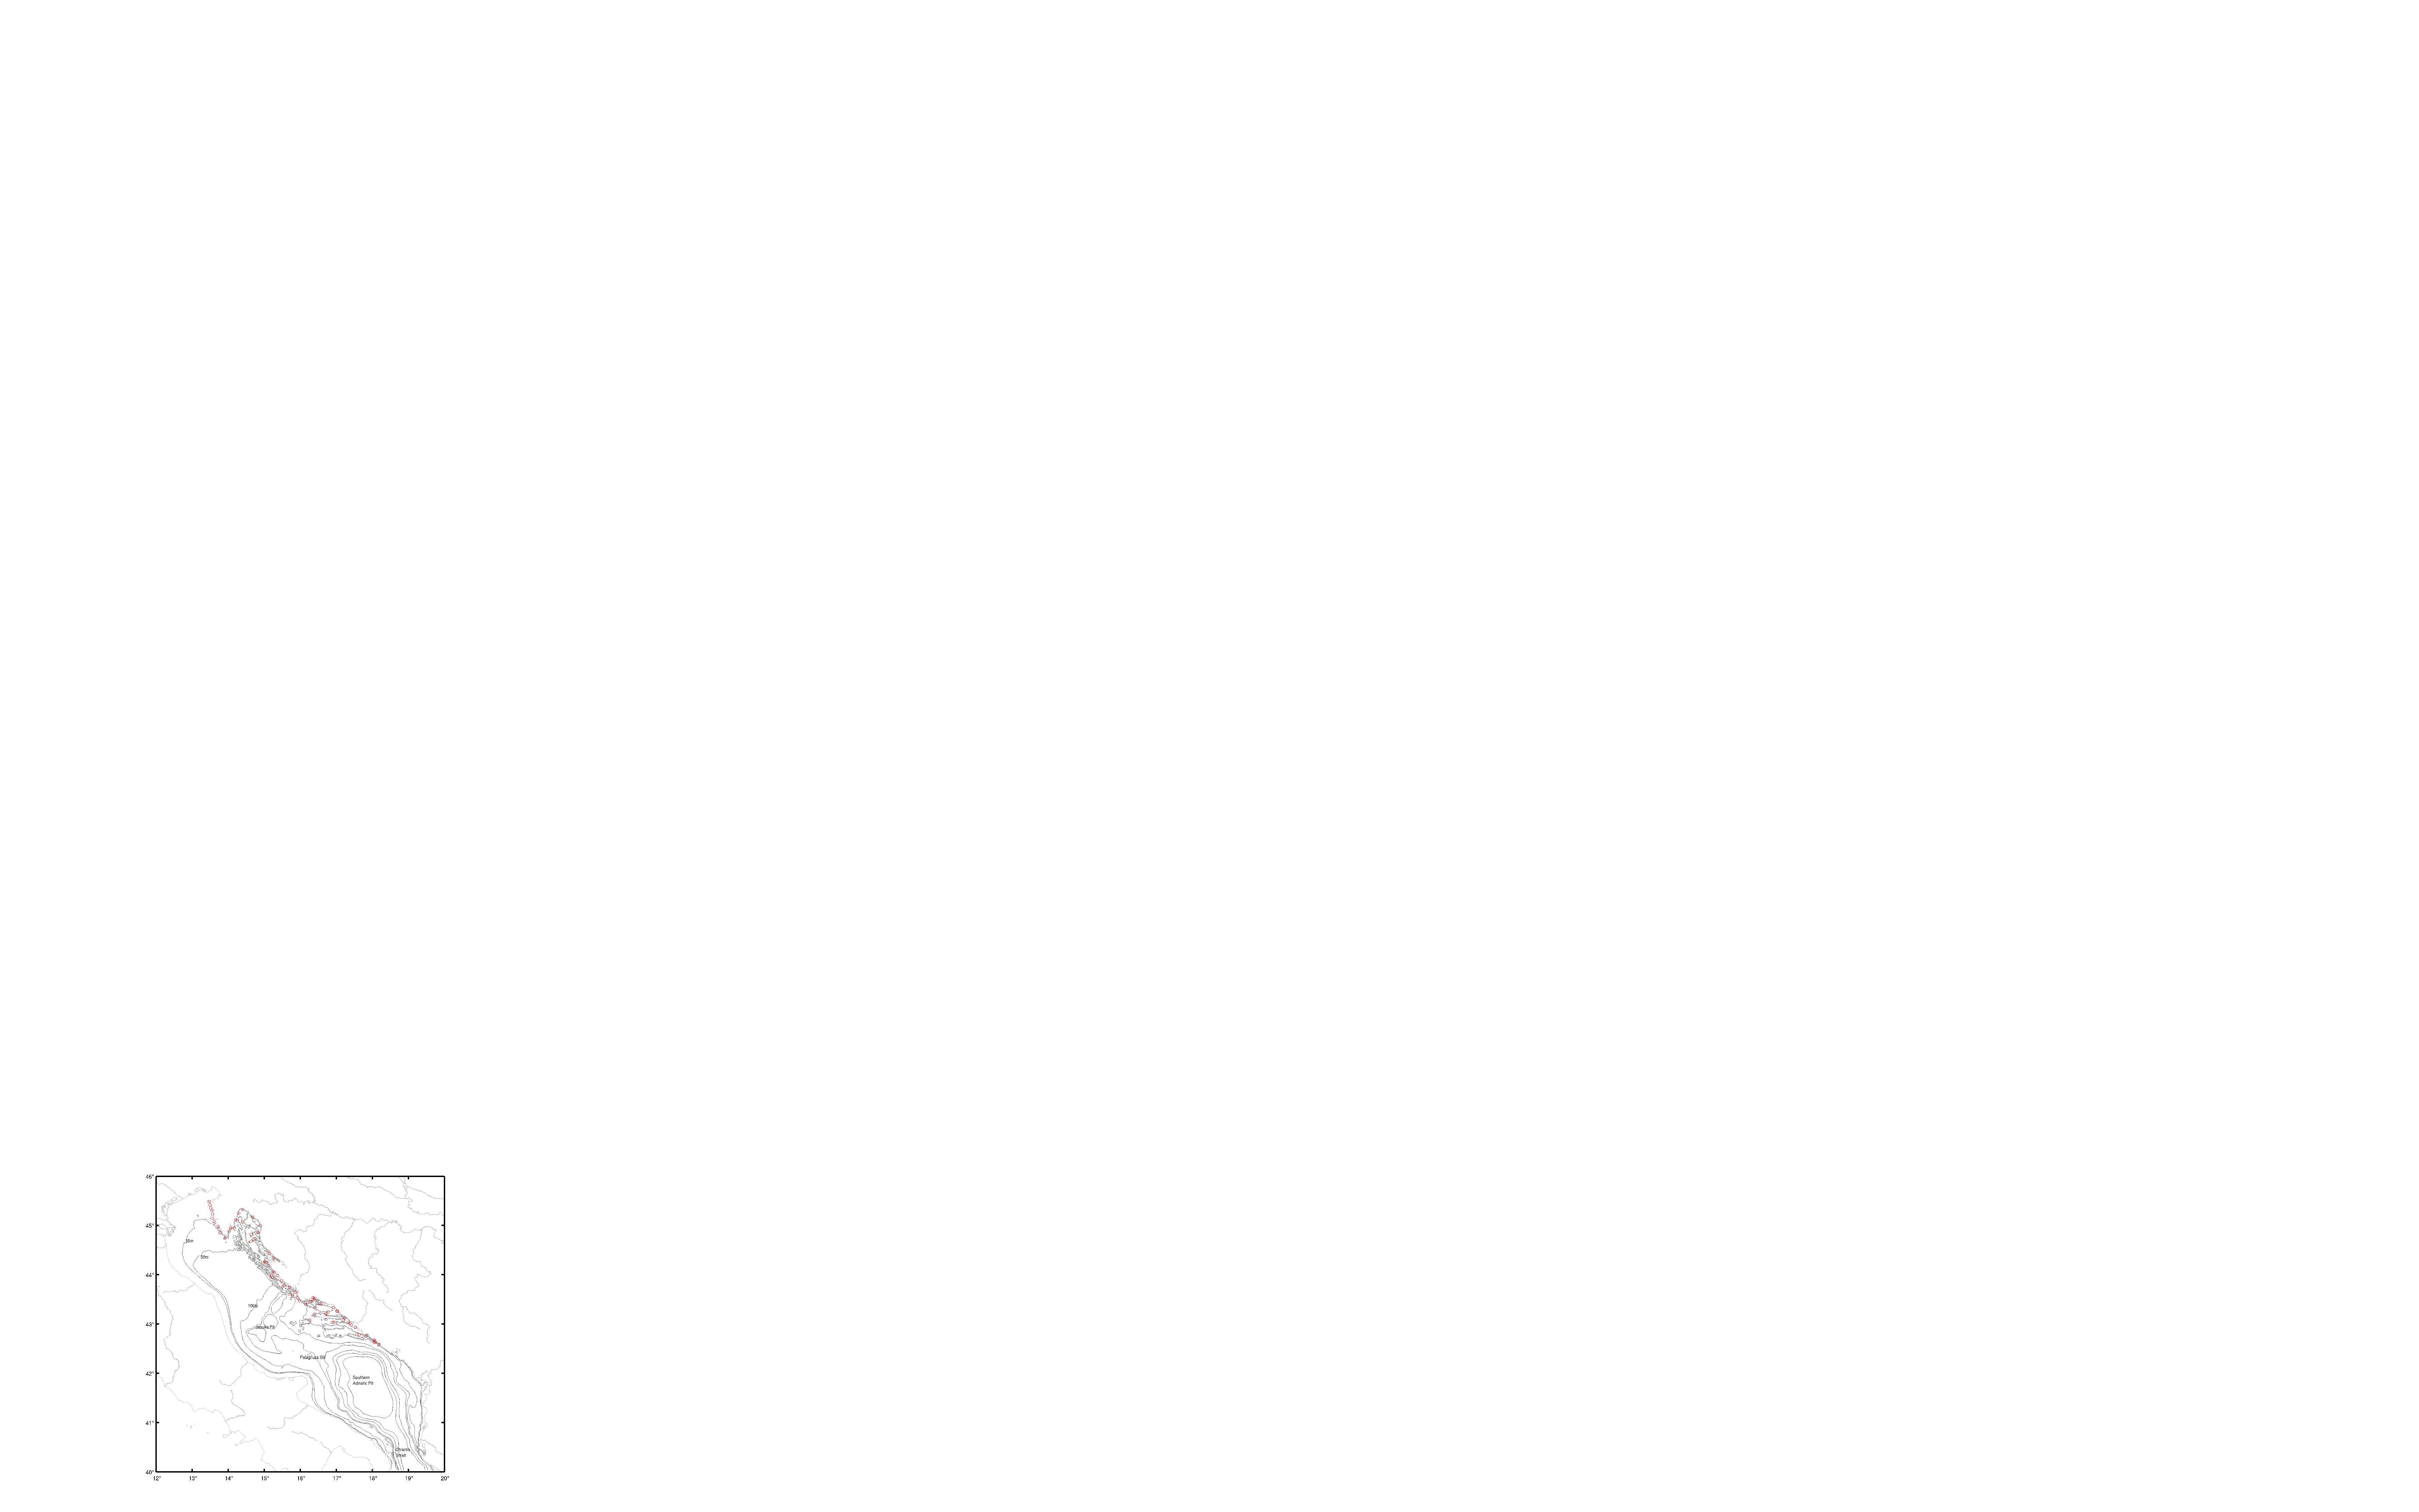
\includegraphics[bb=203 45 628 476, clip]{PictureElect/Stations300_noline.pdf}}\par
%\end{center}
%}


%\frame{
%  \frametitle{Results (\textcolor{blue}{CTD})}
%\begin{itemize}
%\item One problem is that \textcolor{blue}{CTD} measurements are done near the coast, exactly where the model is expected to be bad.
%\item For the \textcolor{blue}{CTD} we found following results:
%\begin{center}
%\begin{tabular}{|c|c|c|c|c|c|c|}
%\hline
%Mean cruise & \multicolumn{2}{|c|}{Temperature (deg)} &\multicolumn{2}{|c|}{Salinity (PSU)}\\
%date        & {\tt RMSE}  & {\tt ME}     &  {\tt RMSE}  & {\tt ME}    \\\hline
%01-11-2007  & 1.18  &  0.84  &  0.47  & -0.17 \\
%20-03-2008  & 0.61  &  0.33  &  0.69  & -0.30 \\
%01-06-2008  & 0.92  & -0.21  &  0.92  & -0.44 \\
%01-07-2008  & 1.38  & -0.37  &  0.79  & -0.41 \\\hline
%\end{tabular}
%\end{center}
%\item Large error for November 2007 is explained by the time of spin up of the model in august 2008.
%\item Summer is generally more difficult to model appropriately due to stronger stratification.
%\item Also problematic for modelling are narrow straits between islands.
%\end{itemize}
%}




%\frame{
%  \frametitle{Comparison with QuikSCAT}
%
%\begin{itemize}
%\item QuikSCAT scatterometer provides sea surface neutral ($10m$) wind field at a $12.5km$ resolution.
%\item When running the ROMS model, the stability contribution are computed and we thus get estimates of neutral winds.
%\item Instrument specification gives zero bias and {\tt RMSE} $2m/s$ and $20deg$ for magnitude and direction.
%Validation studies with {\em in situ} data in coastal region ($<80km$) show larger error ($0.93 \pm 1.83 m/s$) and ($4.71 \pm 31.15 deg$) (Tang et al., 2004).
%\item Validation of ALADIN data with QuikSCAT data shows
%\begin{center}
%speed:   $-1.15 \pm 2.50 m/s$, 
%direction:  $-4.16 \pm  38.14 deg$
%\end{center}
%\end{itemize}

%\begin{center}
%\begin{minipage}{10.2cm}
%\centering
%\resizebox{8.5cm}{!}{\includegraphics[trim=7mm 151mm 7mm 3mm, clip]{FIG_wave/ALD_QS_spatial_comparison.png}}\par
%\end{minipage}
%\begin{minipage}{23.2cm}
%\centering
%\resizebox{23.0cm}{!}{\includegraphics[trim=25mm 25mm 32mm 145mm, clip]{FIG_wav%e/ALD_QS_spatial_comparison.png}}\par
%\end{minipage}
%\end{center}
%}

\frame{
  \frametitle{Comparison with QuikSCAT of ALADIN windspeed}

\begin{center}
\begin{minipage}{5.3cm}
\centering
\resizebox{5.5cm}{!}{\includegraphics{NCLpictures_buoy/DoNCL_ScatterQS/MagScatter.eps}}\par
\end{minipage}
\end{center}
\begin{itemize}
\item Wind speed is systematically underestimated by atmospheric models.
\item Reasons seems to be too small resolution and less sophisticated model than {\tt IFS}.
%\item Problems in direction as well.
\end{itemize}
}





\frame{
  \frametitle{Comparison of Charnock coefficient}
\begin{center}
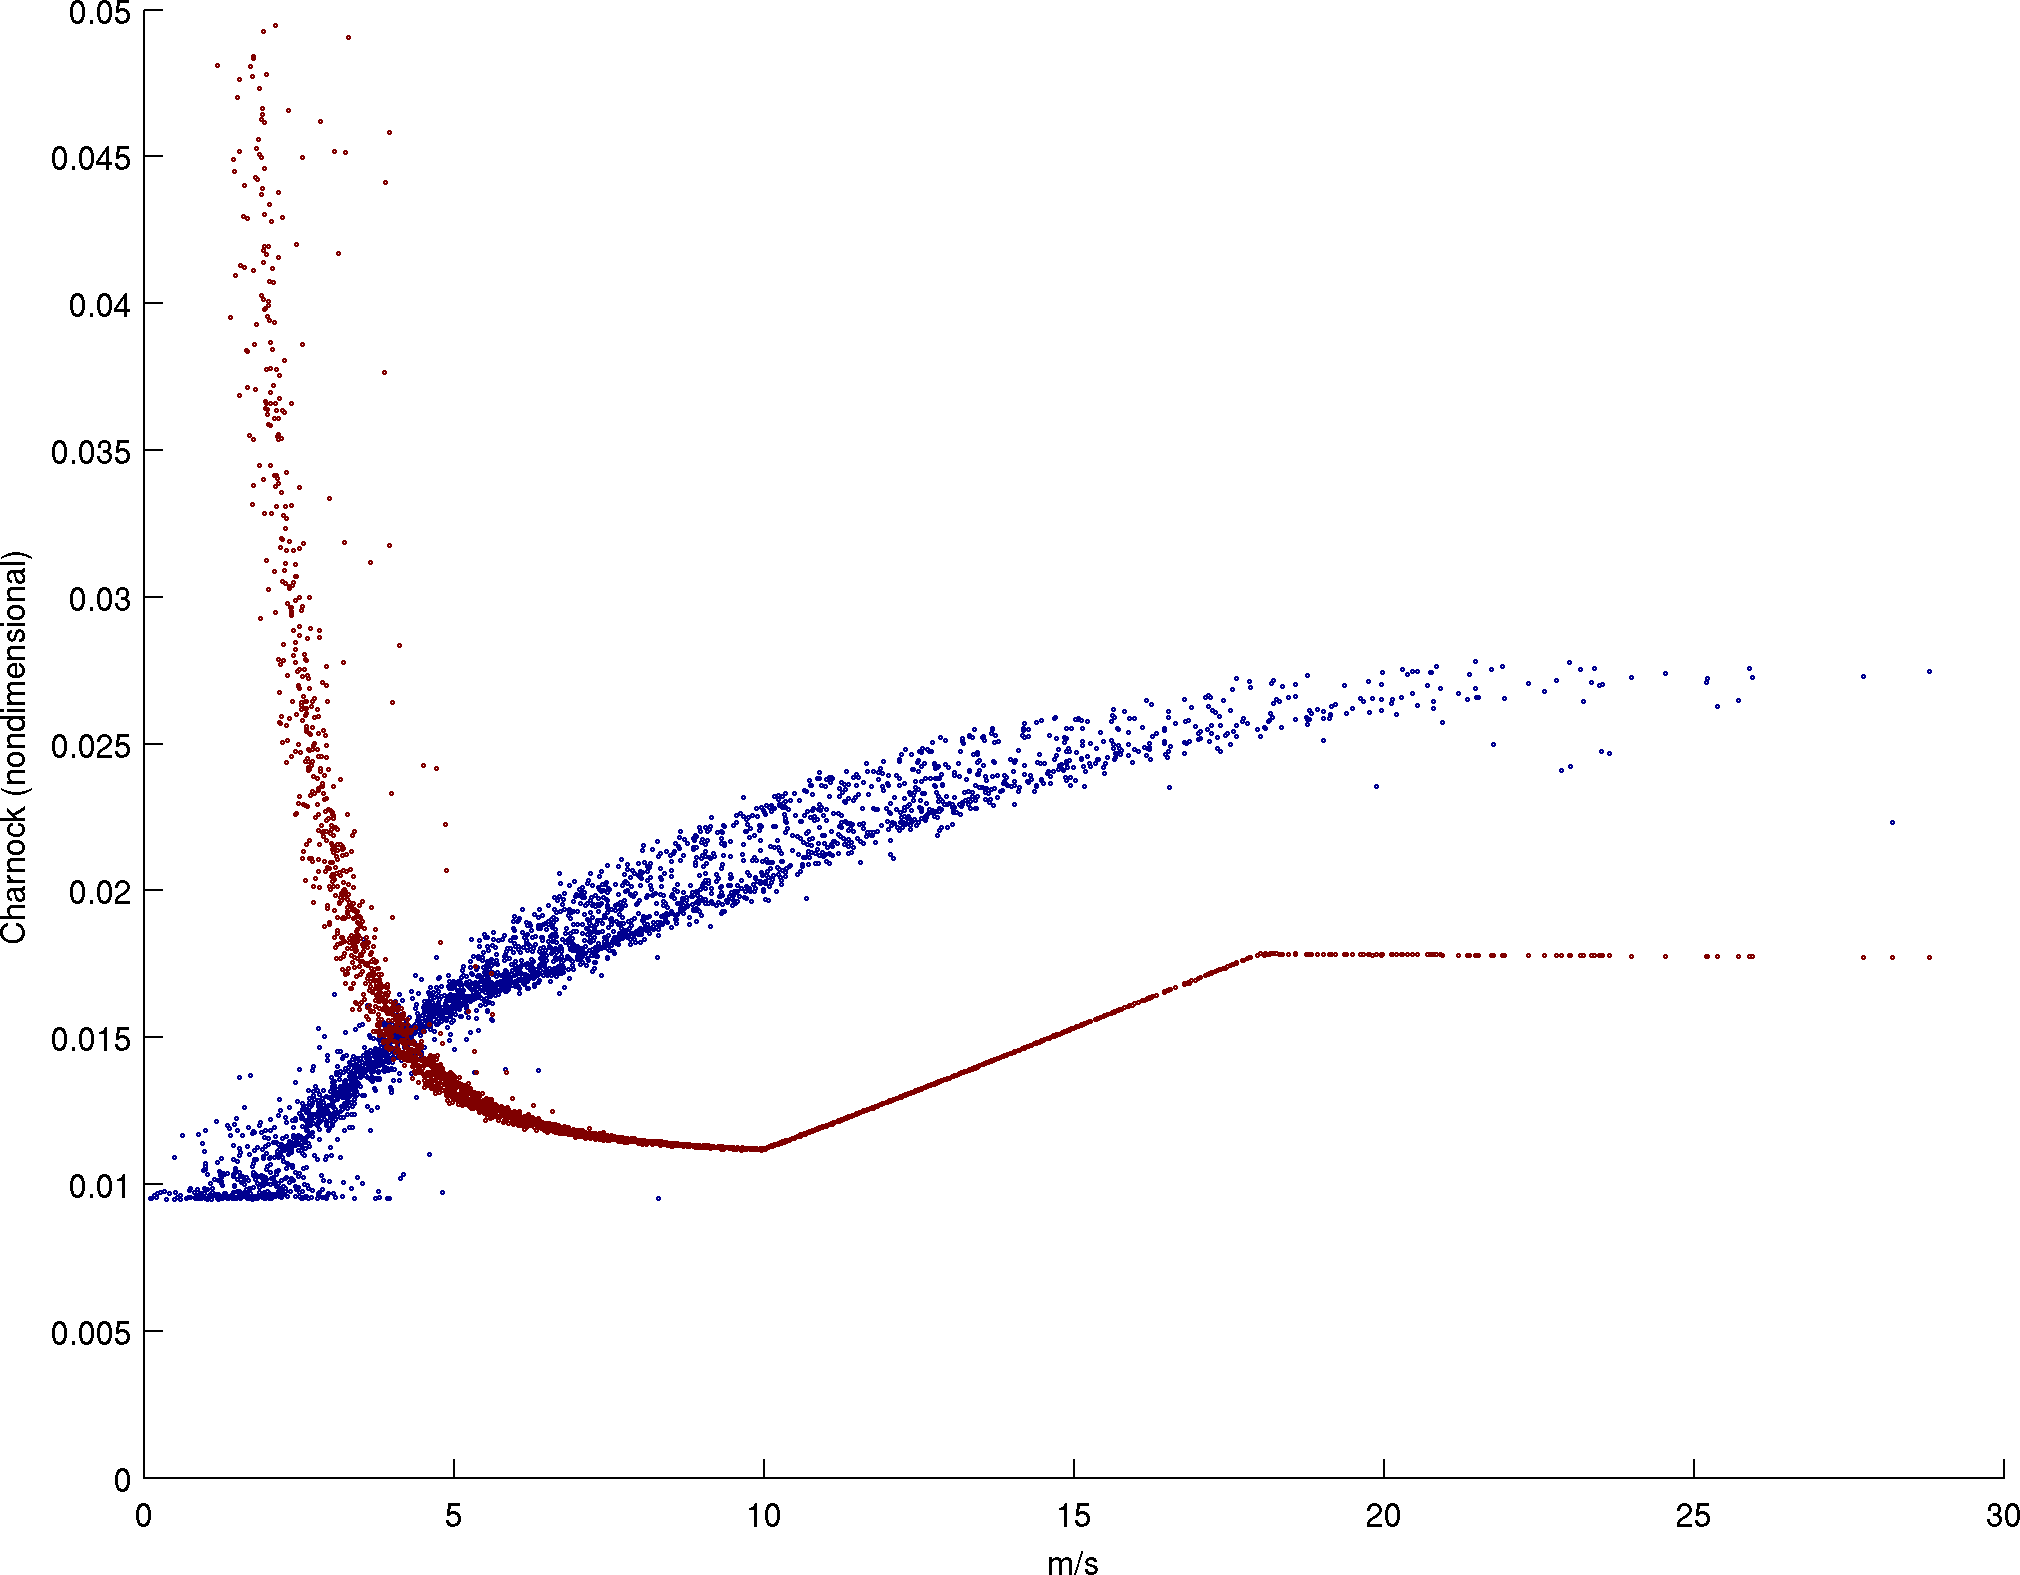
\epsfig{file=DrifterPicture/Scatter_Charnock/Scatter_bulk_wave.png, height=50mm}\par
\end{center}
\begin{itemize}
\item We see that the bulk formulation introduce an artificial looking Charnock coefficient with no spreading.
\item The wave formulation used here is the Ardhuin et al, (2009).
\end{itemize}
}




%\frame{
%  \frametitle{Grids of the Adriatic}
%trim=l b r t
%\begin{center}
%\begin{minipage}{5.2cm}
%\resizebox{5.2cm}{!}{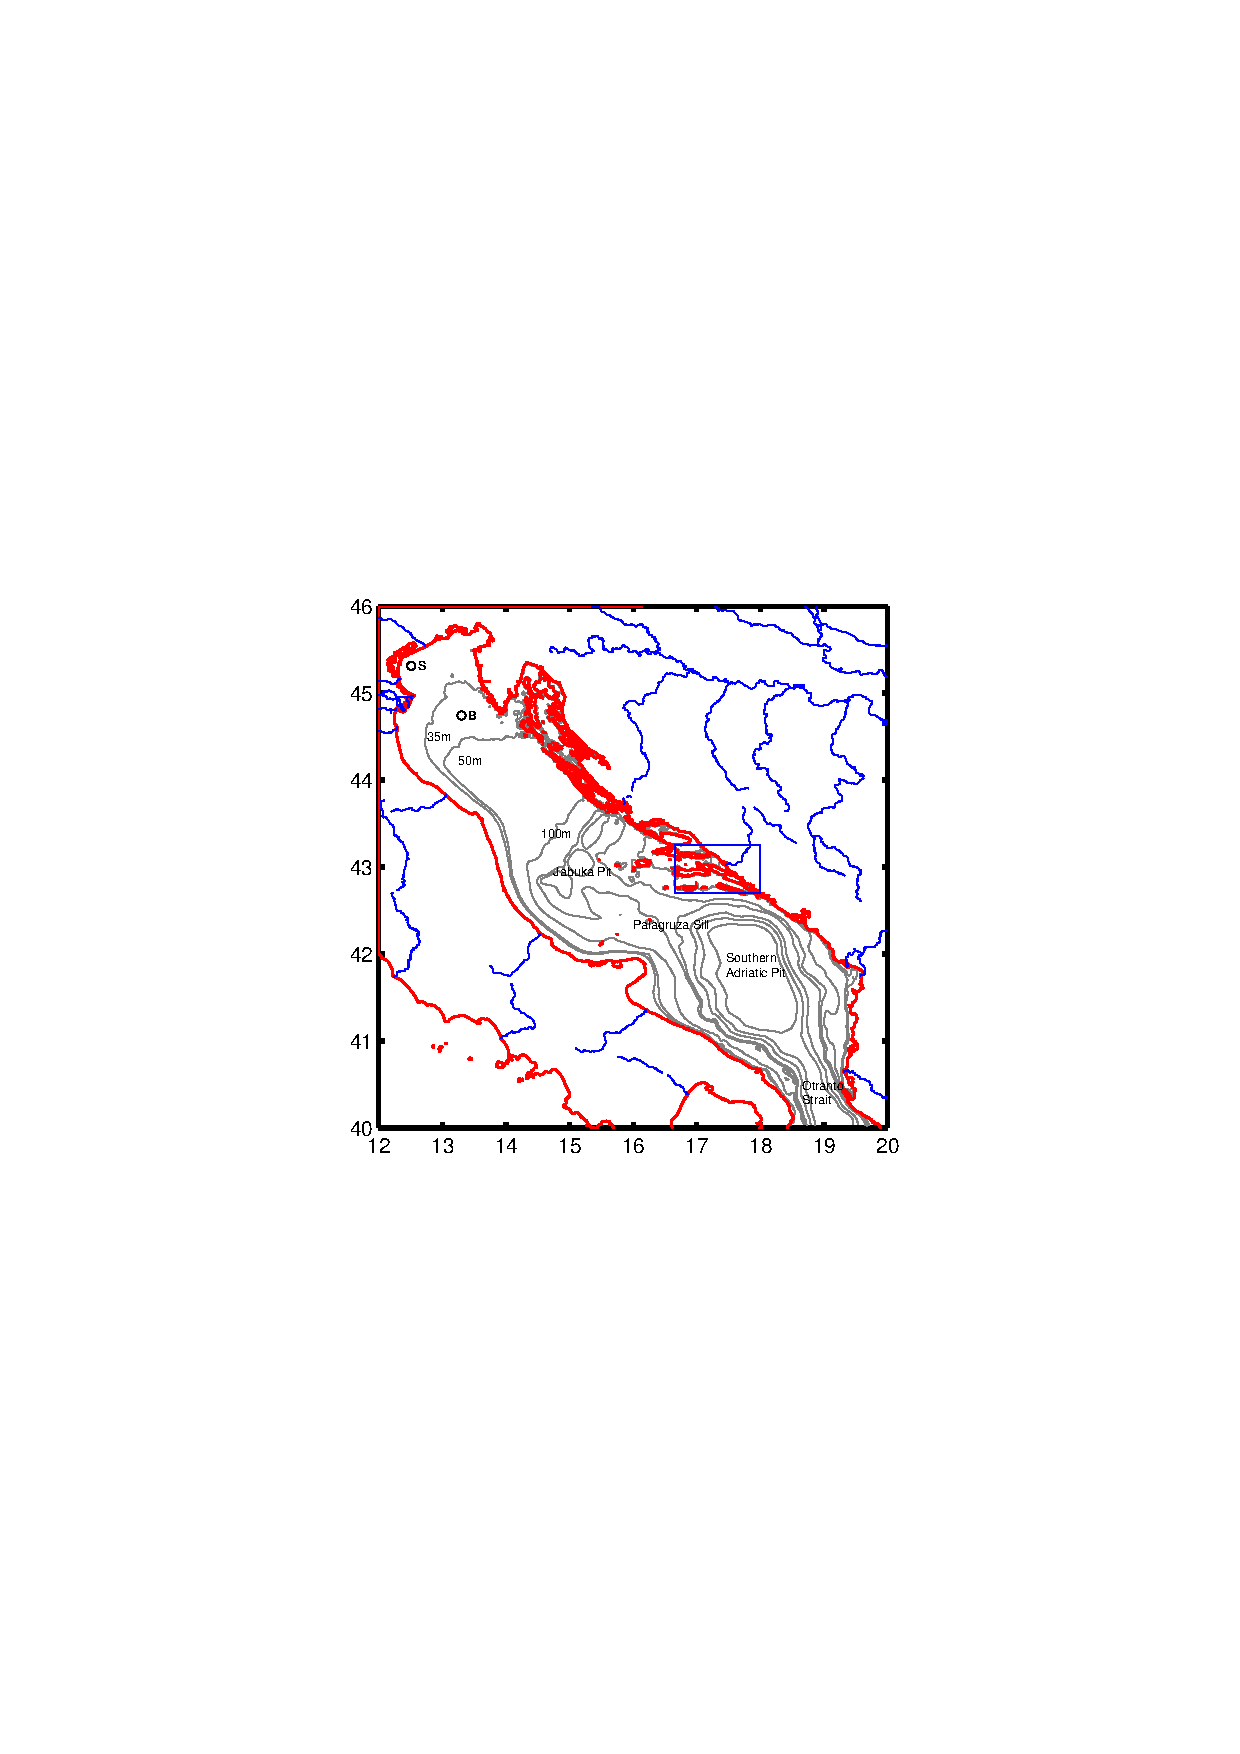
\includegraphics[bb=166 390 399 555,clip]{FIG_wave/Stations300_AASSb.pdf}}\par
%\end{minipage}
%\begin{minipage}{5.2cm}
%\resizebox{6.3cm}{!}{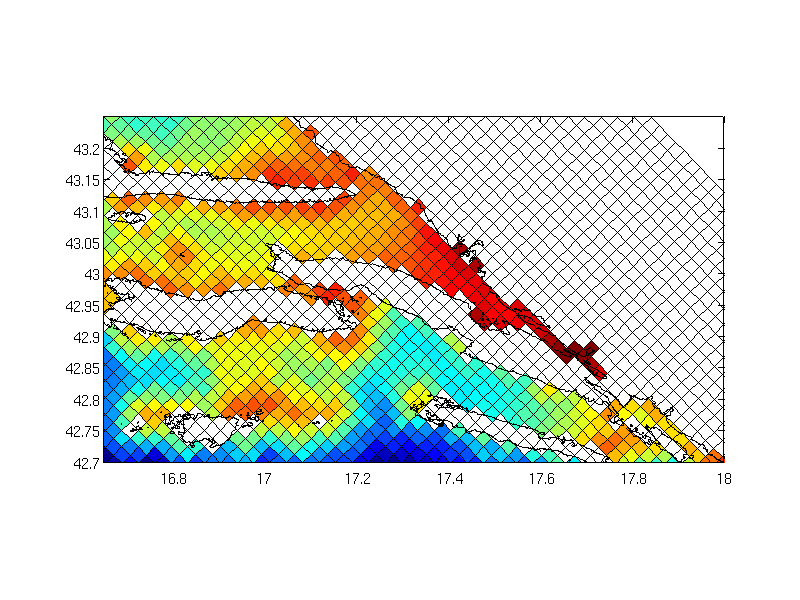
\includegraphics[trim=16mm 28mm 16mm 28mm, clip]{FIG_wave/PicCompar/RomsGrid.png}}\par
%\end{minipage}
%\end{center}
%\begin{center}
%\begin{minipage}{5.2cm}
%\resizebox{5.8cm}{!}{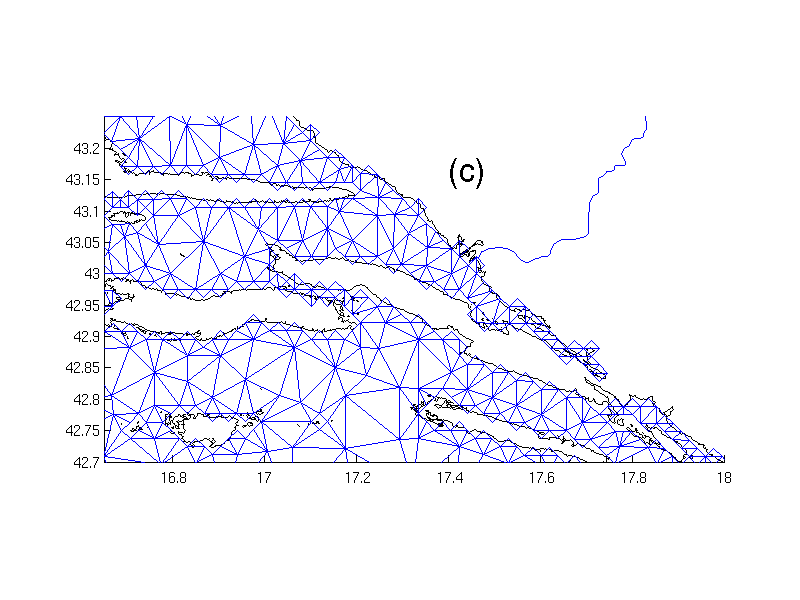
\includegraphics[trim=16mm 28mm 16mm 28mm, clip]{FIG_wave/PicCompar/FEMgrid1.png}}\par
%\end{minipage}
%\begin{minipage}{5.2cm}
%\resizebox{5.8cm}{!}{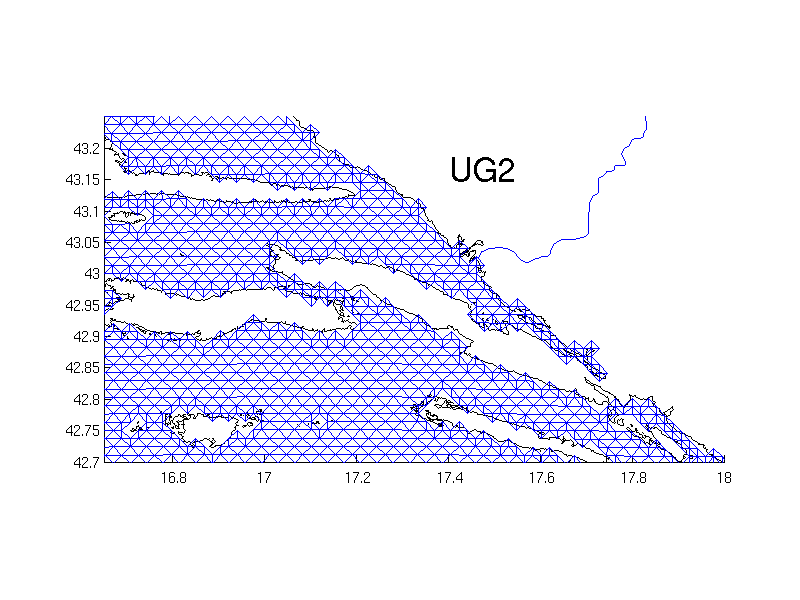
\includegraphics[trim=16mm 28mm 16mm 28mm, clip]{FIG_wave/PicCompar/FEMgrid2.png}}\par
%\end{minipage}
%\end{center}
%}





%\frame{
%  \frametitle{Mean absolute error between grid {\tt UG1} and {\tt UG2} I}
%\begin{center}
%\begin{minipage}{5.3cm}
%\centering
%\resizebox{5.5cm}{!}{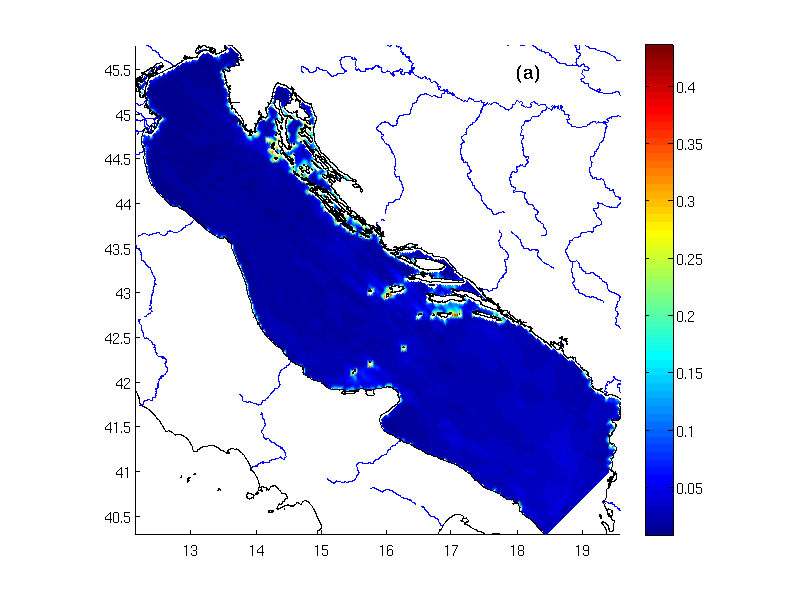
\includegraphics[trim=23mm 10mm 23mm 10mm, clip]{FIG_wave/DiffPictures/HwaveDiff.png}}\par
%Significant wave height
%\end{minipage}
%\begin{minipage}{5.3cm}
%\centering
%\resizebox{5.5cm}{!}{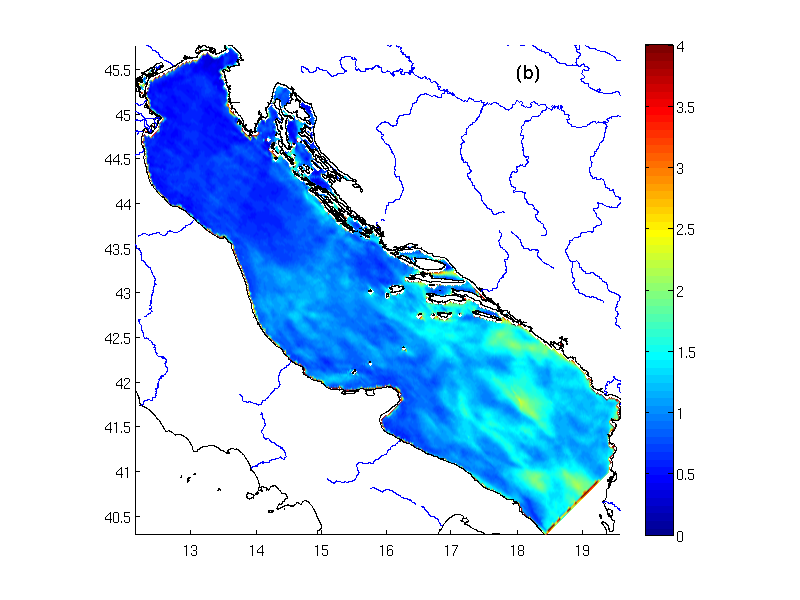
\includegraphics[trim=23mm 10mm 23mm 10mm, clip]{FIG_wave/DiffPictures/LwaveDiff.png}}\par
%Mean wave length
%\end{minipage}
%\end{center}
%\begin{itemize}
%\item The grid impact on Significant wave height is very small.
%\item It is larger for Mean wave length, but still reasonable.
%\end{itemize}
%}

%\frame{
%  \frametitle{Mean absolute error between grid {\tt UG1} and {\tt UG2} II}
%\begin{center}
%\begin{minipage}{5.3cm}
%\centering
%\resizebox{5.5cm}{!}{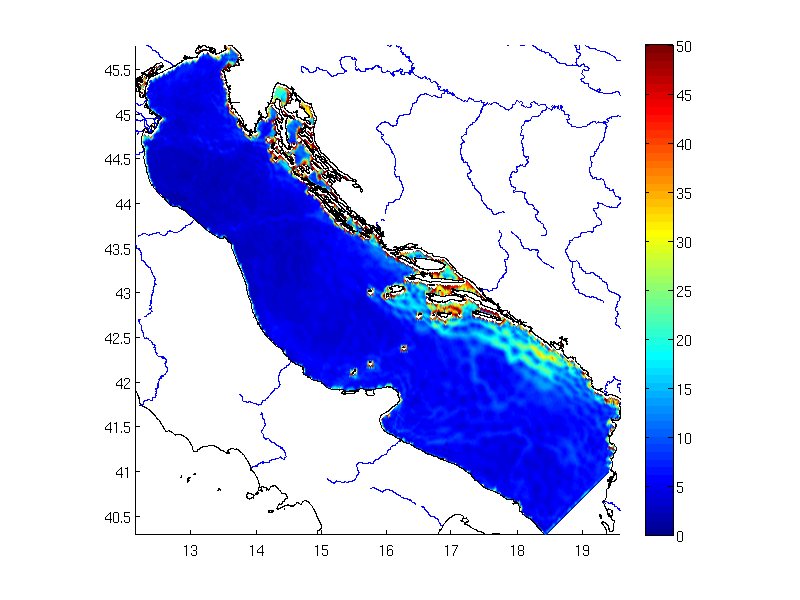
\includegraphics[trim=23mm 10mm 23mm 10mm, clip]{FIG_wave/DiffPictures/DwaveDiff.png}}\par
%Mean wave direction
%\end{minipage}
%\begin{minipage}{5.3cm}
%\centering
%\resizebox{5.5cm}{!}{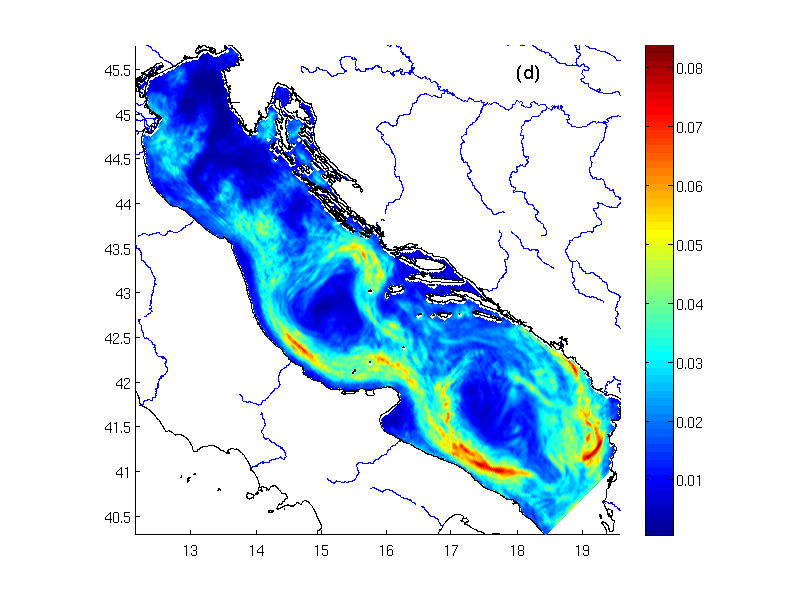
\includegraphics[trim=23mm 10mm 23mm 10mm, clip]{FIG_wave/DiffPictures/UVnormDiff.png}}\par
%Surface current
%\end{minipage}
%\end{center}
%\begin{itemize}
%\item Wind direction is more unstable when the waves are smaller.
%\item For surface current, we see that the Stokes drift is fairly important for the Western Adriatic Current.
%\item The future appears to be to go to unstructured models (Work in preparation with Y. Zhang and A. Roland on coupling of {\tt SELFE} and {\tt WWM}).
%\end{itemize}
%Work done with A. Roland (TU Darmstadt), I. Toma\u zi\'c, I. Janekovi\'c, M. Kuzmi\'c (IRB).
%}

\frame{
  \frametitle{Impact of various parameterizations}

\begin{itemize}
\item The most significant impact of coupling with wave model on surface currents is the parameterization $z_{0,sea} = 0.5 H_s$ of sea roughness length.
\begin{itemize}
\item Reduction of $15$ cm/s of current speed during bora events on the tip of Istria
\end{itemize}
\item The next most significant effect is the effect of GLM formulation with reduction of current speed by $3$ cm/s on the Italian coastline
\item Finally the use of surface stress from the wave model is difficult to assess but leads to further decrease of surface currents in the bora jet.
\end{itemize}
}




\frame{
  \frametitle{Bora event I}
\begin{center}
\begin{minipage}{5.3cm}
\centering
\resizebox{5.5cm}{!}{\includegraphics{NCLpictures_buoy/DoNCL_BoraTime/TheWindB.eps}}\par
\end{minipage}
\begin{minipage}{5.3cm}
\centering
\resizebox{5.5cm}{!}{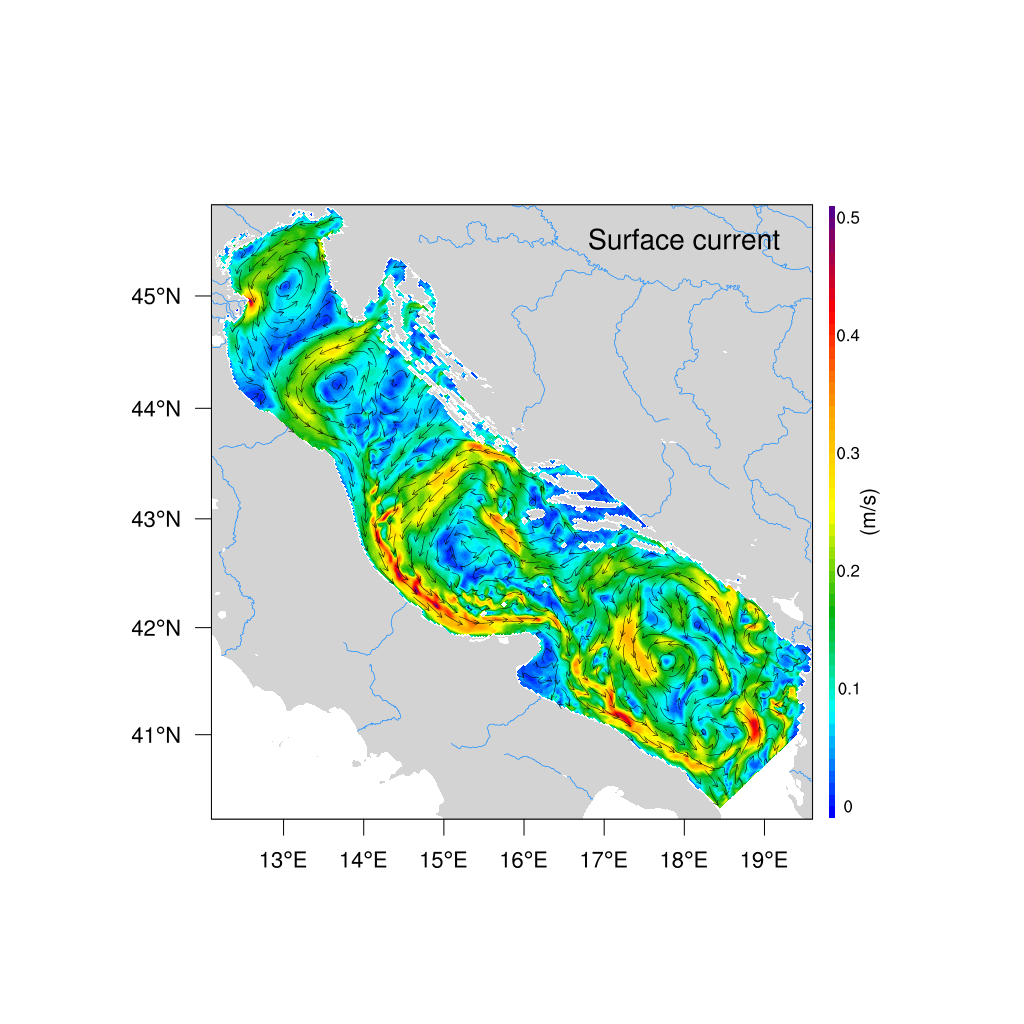
\includegraphics{NCLpictures_buoy/DoNCL_BoraTime/TheCurrentB.eps}}\par
\end{minipage}
\end{center}

\begin{itemize}
\item Wind speed and surface current at 2007-11-17 06:00:00 during a bora event.
\item The bora jets induce a multiple gyre structure on surface currents.
\end{itemize}

}




\frame{
  \frametitle{Bora event II}
\begin{center}
\begin{minipage}{5.3cm}
\centering
\resizebox{5.5cm}{!}{\includegraphics{NCLpictures_buoy/DoNCL_BoraTime/HwaveB.eps}}\par
\end{minipage}
\begin{minipage}{5.3cm}
\centering
\resizebox{5.5cm}{!}{\includegraphics{NCLpictures_buoy/DoNCL_BoraTime/DiffHwaveB.eps}}\par
\end{minipage}
\end{center}

\begin{itemize}
\item Coupling led to a decrease of $H_s$ in the bora jet and an increase outside of the jet due to opposing currents.
\end{itemize}


}



\frame{
  \frametitle{Possible extensions}

\begin{itemize}
\item We did the coupling of COSMO and WAM. Key point is the Charnock coefficient is computed in the WAM model and used by the atmospheric model.
\begin{itemize}
\item The atmospheric model provides the wind and air density to wave model.
\item The wave model provides the Charnock coefficient to the atmospheric model.
\end{itemize}
\item Results on the Mediterranean indicate a slight decrease of wind magnitude and an overall improvements in wave and wind statistics when comparing with altimeter and stations.
\item Further coupling with Atmospheric local model, for example COSMO or WRF.
\item Key issue is the physical parameterization of the sea surface.
\end{itemize}
}





%\frame{
%  \frametitle{Thank you}
%\vspace{1.5cm}
%\begin{center}
%{\Huge \textcolor{red}{T}\textcolor{blue}{H}\textcolor{green}{A}\textcolor{blue}{N}\textcolor{red}{K}}\\[1cm]
%{\Huge \textcolor{red}{Y}\textcolor{blue}{O}\textcolor{red}{U}}
%\epsfig{file=plit-gal10.eps, height=5.5cm}
%\end{center}
%}




\end{document}
